%  LaTeX support: latex@mdpi.com
%  In case you need support, please attach any log files that you could have, and specify the details of your LaTeX setup (which operating system and LaTeX version / tools you are using).

%=================================================================

% LaTeX Class File and Rendering Mode (choose one)
% You will need to save the "mdpi.cls" and "mdpi.bst" files into the same folder as this template file.

%=================================================================

\documentclass[sensors,article,submit,moreauthors,pdftex,12pt,a4paper]{mdpi}
%--------------------
% Class Options:
%--------------------
% journal
%----------
% Choose between the following MDPI journals:
% actuators, administrativesciences, aerospace, agriculture, agronomy, algorithms, animals, antibiotics, antibodies, antioxidants, appliedsciences, arts, atmosphere, atoms, axioms, batteries, behavioralsciences, bioengineering, biology, biomedicines, biomimetics, biomolecules, biosensors, brainsciences, buildings, cancers, catalysts, cells, challenges, chemosensors, children, chromatography, climate, coatings, computation, computers, cosmetics, crystals, data, dedntistryjournal, diagnostics, diseases, diversity, econometrics, economies, education, electronics, energies, entropy, environmentalsciences, environments, epigenomes, fibers, foods, forests, futureinternet, galaxies, games, gels, genealogy, genes, geosciences, healthcare, horticulturae, humanities, hydrology, informatics, information, inorganics, insects, ijerph, ijfs, ijms, ijgi, jcdd, jcm, jdb, jfb, jimaging, jof, joi, jlpea, jmse, jpm, jrfm, jsan, land, laws, life, lubricants, machines, marinedrugs, materials, mathematics, medicalsciences, membranes, metabolites, metals, microarrays, micromachines, microorganisms, minerals, molbank, molecules, nanomaterials, ncrna, nutrients, pathogens, pharmaceuticals, pharmaceutics, pharmacy, photonics, plants, polymers, processes, proteomes, publications, religions, remotesensing, resources, risks, robotics, safety, sensors, sinusitis, socialsciences, societies, sports, standards, sustainability, symmetry, systems, technologies, toxics, toxins, universe, vaccines, veterinarysciences, viruses, water
%---------
% article
%---------
% The default type of manuscript is article, but could be replaced by using one of the class options:
% article, review, communication, commentary, bookreview, correction, addendum, editorial, changes, supfile, casereport, comment, conceptpaper, conferencereport, meetingreport, discussion, essay, letter, newbookreceived, opinion, projectreport, reply, retraction, shortnote, technicalnote, creative, datadescriptor (for journal Data)
%----------
% submit
%----------
% The class option "submit" will be changed to "accept" by the Editorial Office when the paper is accepted. This will only make changes to the frontpage (e.g. the logo of the journal will get visible), the headings, and the copyright information. Journal info and pagination for accepted papers will also be assigned by the Editorial Office.
% Please insert a blank line is before and after all equation and eqnarray environments to ensure proper line numbering when option submit is chosen
%------------------
% moreauthors
%------------------
% If there is only one author the class option oneauthor should be used. Otherwise use the class option moreauthors.
%---------
% pdftex
%---------
% The option "pdftex" is for use with pdfLaTeX only. If eps figure are used, use the optioin "dvipdfm", with LaTeX and dvi2pdf only.

%=================================================================
\setcounter{page}{1}
\lastpage{x}
\doinum{10.3390/------}
\pubvolume{xx}
\pubyear{2015}
%\externaleditor{Academic Editor: xx}
\history{Received: xx / Accepted: xx / Published: xx}
%------------------------------------------------------------------
% The following line should be uncommented if the LaTeX file is uploaded to arXiv.org
%\pdfoutput=1

%=================================================================

% Add packages and commands to include here
% The amsmath, amsthm, amssymb, hyperref, caption, float and color packages are loaded by the MDPI class.
\usepackage{graphicx}
\usepackage[caption=false]{subfig}
%\usepackage{subfigure,psfig}

\usepackage[utf8]{inputenc} % for use umulaut
\usepackage{textcomp}	% for use Trademarks symbol

\usepackage{booktabs}
\newcommand{\bigcell}[1]{\shortstack[l]{#1}}

\usepackage{multirow,tabularx}
\newcolumntype{Y}{>{\centering\arraybackslash}X}

\usepackage{amsmath}
\usepackage{algorithm}
\usepackage[noend]{algpseudocode}
\algdef{SE}[DOWHILE]{Do}{doWhile}{\algorithmicdo}[1]{\algorithmicwhile\ #1}%
\renewcommand{\algorithmiccomment}[1]{\hfill\bgroup//~#1\egroup}
\algnewcommand{\LineComment}[1]{\State // #1}

\newcommand{\JHMEMO}[1]{\textcolor{red}{#1}}

\newcolumntype{L}[1]{>{\raggedright\arraybackslash}p{#1}}
\newcolumntype{C}[1]{>{\centering\arraybackslash}p{#1}}
\newcolumntype{R}[1]{>{\raggedleft\arraybackslash}p{#1}}

% \setcounter{secnumdepth}{5}

%=================================================================
%% Please use the following mathematics environments:
% \theoremstyle{mdpi}
% \newcounter{thm}
% \setcounter{thm}{0}
% \newcounter{ex}
% \setcounter{ex}{0}
% \newcounter{re}
% \setcounter{re}{0}
%
% \newtheorem{Theorem}[thm]{Theorem}
% \newtheorem{Lemma}[thm]{Lemma}
% \newtheorem{Corollary}[thm]{Corollary}
% \newtheorem{Proposition}[thm]{Proposition}
%
% \theoremstyle{mdpidefinition}
% \newtheorem{Characterization}[thm]{Characterization}
% \newtheorem{Property}[thm]{Property}
% \newtheorem{Problem}[thm]{Problem}
% \newtheorem{Example}[ex]{Example}
% \newtheorem{ExamplesandDefinitions}[ex]{Examples and Definitions}
% \newtheorem{Remark}[re]{Remark}
% \newtheorem{Definition}[thm]{Definition}
%% For proofs, please use the proof environment (the amsthm package is loaded by the MDPI class).

%=================================================================

% Full title of the paper (Capitalized)
\Title{Fast Contour-Tracing Algorithm based on Pixel-Following Method for Contour Representation}

% Authors (Add full first names)
\Author{Jonghoon Seo$^{1,\dagger}$,  Seungho Chae$^{1,\dagger}$, Jinwook Shin $^{1,\dagger}$, Dongchul Kim $^{1,\dagger}$, Cheolho Cheong$^{1,\dagger}$ and Tack-Don Han $^{1,}$*}

% Affiliations / Addresses (Add [1] after \address if there is only one affiliation.)
\address{%
$^{1}$ Department of Computer Science, Yonsei University, 134 Sinchon-dong Seodaemun-gu, Seoul, Republic of Korea}

\contributed{$^\dagger$ These authors contributed equally to this work.}

% Contact information of the corresponding author (Add [2] after \corres if there are more than one corresponding author.)
\corres{hantack55@msl.yonsei.ac.kr, +82-2-2123-2715 and +82-2-365-2579}

% Abstract (Do not use inserted blank lines, i.e. \\)
% \abstract{This is the abstract section. The abstract should be one section and count less than 200 words.}
%!TEX root = ../Fast_Contour_Tracing_Algorithm.tex
% -*- root: ../Fast_Contour_Tracing_Algorithm.tex -*-

\abstract{In this paper, we present a novel contour tracing algorithm based on the pixel following method for fast and accurate contour following. The proposed algorithm distinguishes between types of contour such as a local pattern type based on its relative location among several contour pixels, and then it traces the next contour pixel by using the previous. Therefore, it can classify the type of contour pixels into straight line, inner corner, outer corner, and inner-outer corner, and it can extract pixels of a specific contour type. Moreover, it can trace contour pixels rapidly because it can determine the local minimal path using the contour case. In addition, the proposed algorithm has the ability to compress data of contour pixels by using the representative points and inner-outer corner points, and it can also accurately restore the contour image from the data. To compare the performance of the proposed algorithm with that of conventional techniques, we measured their processing time and accuracy. In the experimental results, the proposed algorithm shows better performance when compared to the others, and it can provide compressed data of contour pixels and restore them accurately, including the inner-outer corner that cannot be restored using conventional algorithms.}



% Keywords: add 3 to 10 keywords
\keyword{Contour tracing; boundary following; pixel following; vertex following; contour restoration; contour representation}

% The fields PACS, MSC, and JEL may be left empty or commented out if not applicable
%\PACS{}
%\MSC{}
%\JEL{}

% If this is an expanded version of a conference paper, please cite it here: enter the full citation of your conference paper, and add $^\dagger$ in the end of the title of this article.
%\conference{}

%%%%%%%%%%%%%%%%%%%%%%%%%%%%%%%%%%%%%%%%%%
% For journal Data:

%\dataset{DOI number or link to the deposited data set in cases where the data set is published or set to be published separately. If the data set is submitted and will be published as a supplement to this paper in the journal Data, this field will be filled by the editors of the journal. In this case, please make sure to submit the data set as a supplement when entering your manuscript into our manuscript editorial system.}
%\datasetlicense{license under which the data set is made available (CC0, CC-BY, CC-BY-SA, CC-BY-NC, etc.)}

%%%%%%%%%%%%%%%%%%%%%%%%%%%%%%%%%%%%%%%%%%

\begin{document}

%!TEX root = ../Fast_Contour_Tracing_Algorithm.tex
% -*- root: ../Fast_Contour_Tracing_Algorithm.tex -*-

\section{Introduction}

% A contour is defined as a segment that is one pixel wide and one or more pixels in length, and a boundary is defined as an unbroken contour\cite{Mcqueen2004Contour}. Contours and boundaries are very important information for object representation and image recognition. For example, they are used to separate objects from the background, to calculate the size of an object, to classify a shape, and to find the feature points of an object using the length and shape from its contour pixels\cite{Pratt????Digital,Gose1996Pattern}. Moreover, using the contour information, it is possible to save the shape of objects and restore them to their original shapes for various applications in the field of graphics and vision. Therefore, many researches on contour tracing algorithms for extracting and tracing the contour of an object have been conducted. Most of the algorithms are binary-image-based contour tracing algorithms \cite{Pitas2000Digital,Gose1996Pattern,Das1990Bivariate,Papert1973Uses,Cheong2006Improved,Mirante1982Radial,Pavlidis2012Algorithms}, which trace contours on digitized black-and-white images. Moreover, the focus is on contour tracing algorithms based on color images and gray images []; further, the binary-image-based contour tracing algorithm can be easily applied to color and gray images.

A contour is defined as a segment that is one pixel wide and one or more pixels in length, and a boundary is defined as an unbroken contour \cite{Mcqueen2004Contour}. Contours and boundaries provide very important information for object representation and image recognition. For example, they are used to separate objects from their backgrounds, calculate the sizes of objects, classify shapes, and find the feature points of objects using the length and shape of their contour pixels \cite{Pratt????Digital,Gose1996Pattern}. Moreover, in the field of graphics and vision, it is possible to use the contour information to save the shape of objects and restore them to their original shapes for various applications. Therefore, there have been many studies on contour-tracing algorithms for extracting and tracing the contour of an object. Most of the algorithms are binary-image-based contour-tracing algorithms \cite{Pitas2000Digital,Gose1996Pattern,Das1990Bivariate,Papert1973Uses,Cheong2006Improved,Mirante1982Radial,Pavlidis2012Algorithms}, which trace contours on digitized black-and-white images taken from various image sensors.

% In recent years, as the popularity of camera equipped mobile devices such as mobile phones and personal digital assistants (PDAs) has increased, various real-time applications such as image code recognition, face recognition, optical character recognition (OCR), logo recognition, augmented reality (AR), and mixed reality (MR) have emerged for mobile computing environments [], [], []. Since mobile devices possess restricted hardware resources such as low-performance processors, small-sized memory, low-resolution display, and low battery capacity, that require simpler and faster algorithms for image processing. 

In recent years, with the increasing popularity of smart/wearable mobile sensor devices \cite{Aroca2013Wearable} such as smart phones, smart watch and smart glass, various real-time applications such as image code recognition, face recognition, optical character recognition (OCR), logo recognition, augmented reality (AR), and mixed reality (MR) have emerged for sensor computing\cite{Wakaumi20062D,Brodic2010Basic,Kim2006Rapid,Tian2010RealTime,Zhang2012Robust}. Because smart/wearable mobile sensor devices possess limited hardware resources such as low-performance processors, small-sized memory, low-resolution displays, and low battery capacity, they require simpler and faster algorithms for image processing. 

% Generally, a contour tracing algorithm can be evaluated on the basis of the following four criteria: (1) accuracy of contour tracing, (2) processing time, (3) data size to save the traced contour information, and (4) the ability to accurately restore and enlarge the original contour using the saved data. However, there have been few studies on contour tracing algorithms that have sought to satisfy all these criteria. Some of the conventional algorithms miss contour pixels on specific relative pixel locations, and the others require considerable operation time for tracing the pixels because a shortcut to the local patterns is not considered \cite{Cheong2006Improved,Cheong2012Advanced}. Moreover, most of the algorithms have no data compression ability for saving the contour information, and some of them cannot restore the image perfectly using the saved data \cite{Miyatake1997Contour}. 

Generally, a contour tracing algorithm can be evaluated based on the following four criteria: (1) accuracy of contour tracing, (2) processing time, (3) data size to save the traced contour information, and (4) the ability to accurately restore and enlarge the original contour using the saved data. However, few studies on contour-tracing algorithms have sought to satisfy all of these criteria. Some of the conventional algorithms miss contour pixels that are at specific relative pixel locations, and others require considerable processing time to trace the pixels because shortcuts to the local patterns are not considered \cite{Cheong2006Improved,Cheong2012Advanced}. Moreover, most of the algorithms have no data-compression capabilities that enable them to save the contour information, and some of them cannot restore the image perfectly using the saved data \cite{Miyatake1997Contour}. 

% In this paper, we propose a novel contour tracing algorithm based on pixel following that overcomes the abovementioned problems, i.e., (1) it provides fast and accurate results for contour pixel tracing, (2) contour information can be compressed for reducing the memory size, and (3) it accurately restores the compressed data to the original contour image. In order to achieve the objectives, the proposed algorithm initially distinguishes the local patterns made by adjacent contour pixels, then finds next contour pixel will be traced from the pattern. 

In this paper, we propose a novel contour-tracing algorithm based on pixel following that overcomes the abovementioned problems, i.e., (1) it provides fast and accurate results for contour-pixel tracing, (2) contour information can be compressed to reduce the memory size, and (3) it accurately restores the compressed data to the original contour image. In order to achieve the objectives, the proposed algorithm initially distinguishes the local patterns made by adjacent contour pixels, and it then finds the next contour pixel that will be traced from the pattern. 

% The paper is organized as follows. In the next section, conventional contour tracing algorithms are categorized and their characteristics are introduced. Subsequently, we analyze their performance on the basis of accuracy and speed of the contour tracing process, and then the proposed algorithm is described and its contour tracing procedure, data compression technique, and restoration technique are presented. After that, the comparison of the conventional algorithms and the proposed algorithm on the basis of performance is presented along with experimental results that comprise the number of traced pixels and the processing times for real-time large-sized images. Moreover, the compressed data size and its restored results are compared with the original traced contour pixels. Finally, we summarize the characteristics and experimental results of the proposed algorithm.

The paper is organized as follows. In the next section, we categorize conventional contour-tracing algorithms and introduce their characteristics. Subsequently, we analyze their performance based on the accuracy and speed of the contour-tracing process, and we then describe the proposed algorithm, after which we present its contour-tracing procedure, data-compression technique, and restoration technique. Then,, we present a comparison of the conventional algorithms and the proposed algorithm on the basis of their performance, along with experimental results that include the number of traced pixels and the processing times for real-time large-sized images. Moreover, we compare the compressed data size and its restored results with the original traced contour pixels. Finally, we summarize the characteristics and experimental results of the proposed algorithm.
%!TEX root = ../Fast_Contour_Tracing_Algorithm.tex
% -*- root: ../Fast_Contour_Tracing_Algorithm.tex -*-

\section{Related Works}

% Most conventional contour tracing algorithms run on two-dimensional (2D) binary images that consist of black-and-white pixels, which are obtained through binarization, for determining whether a pixel has dark or light intensity. In the digitized image, we can assume that the objects have black pixels and the background has white pixels; therefore, a contour pixel is black and it has at least one adjacent pixel that is white.

To determine whether a pixel has a dark or light intensity, most conventional contour-tracing algorithms are used to process two-dimensional (2D) binary images that consist of black-and-white pixels that are obtained through binarization. In the digitized image, we can assume that the objects have black pixels and the background has white pixels; therefore, a contour pixel is black and it has at least one adjacent pixel that is white.

\subsection{Overview}

%%% Image 1
\begin{figure}[htbp]
	\centering
	\subfloat[]{ 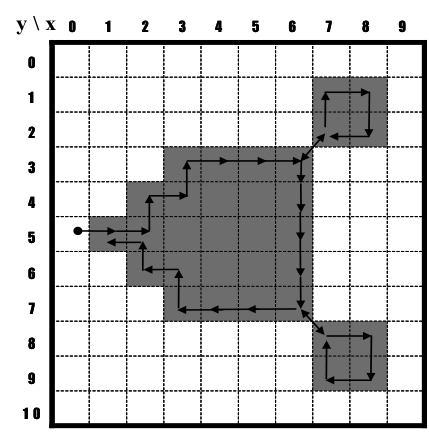
\includegraphics[width=0.3\textwidth, height=5cm]{2.RelatedWorks/fig1-a.png} \label{fig:img1-a} }
	\subfloat[]{ 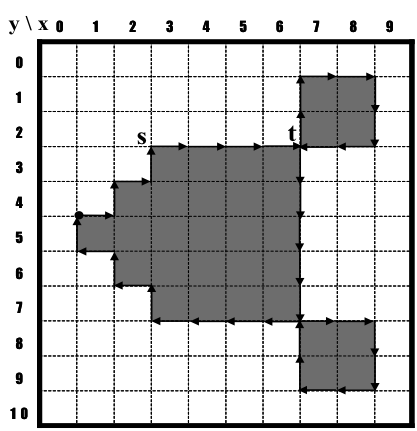
\includegraphics[width=0.3\textwidth, height=5cm]{2.RelatedWorks/fig1-b.png} \label{fig:img1-b} }
	\subfloat[]{ 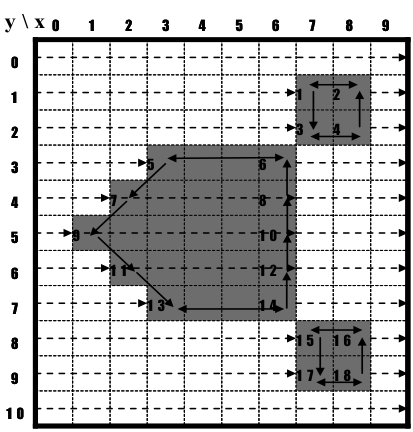
\includegraphics[width=0.3\textwidth, height=5cm]{2.RelatedWorks/fig1-c.png} \label{fig:img1-c} }
	 
	\caption{Contour tracer. \protect\subref{fig:img1-a} Pixel following algorithm \protect\subref{fig:img1-b} Vertex following algorithm \protect\subref{fig:img1-c} Run-data-based following algorithm}
	\label{fig:image1}
\end{figure}

% Figure \ref{fig:image1} shows examples of contour traces obtained by using the contour tracing algorithms. The conventional contour algorithms can be categorized typically into three types as follows: pixel following, vertex following, and run-data-based following \cite{Miyatake1997Contour,Danielsson1981Improvement,Shoji1999Contour}. Among these, the pixel following method is most the common.

Figure \ref{fig:image1} shows examples of contour traces that were obtained using the contour-tracing algorithms. The conventional contour algorithms can typically be categorized into three types as follows: pixel following, vertex following, and run-data-based following \cite{Miyatake1997Contour,Danielsson1981Improvement,Shoji1999Contour}. Of these, the pixel-following method is the most common.

\subsubsection{Pixel-following Method}

The pixel following method traces contour pixels in a predefined manner and then saves their coordinates in the memory according to the trace order. In figure \ref{fig:img1-a}, the algorithm traces contour pixels along the clockwise direction from the current pixel, i.e., it sequentially searches adjacent black pixels of the current pixel using a relative directional order such as left, front-left, front, front-right, right, right-rear, and rear. Pixel following methods such as simple boundary follower (SBF) \cite{Pitas2000Digital,Das1990Bivariate,Papert1973Uses}, modified SBF (MSBF)\cite{Gose1996Pattern}, improved SBF (ISBF)\cite{Cheong2006Improved}, Moore-Neighbor tracing (MNT) \cite{Toussaint????Grids}, modified MNT (MMNT) \cite{Pradhan2010Contour}, radial sweep algorithm (RSA) \cite{Mirante1982Radial}, and Theo Pavlidis algorithm (TPA)\cite{Pavlidis2012Algorithms} have simple rules for tracing contour pixels based on a chain code. On the contrary, this method requires frame size memory to trace the contour, and it also generates erroneous images when the contour image is enlarged\cite{Miyatake1997Contour} since it maintains only the pixel coordinates.

The pixel-following method traces contour pixels in a predefined manner, and then saves their coordinates in memory according to the trace order. In Figure \ref{fig:img1-a}, the algorithm traces contour pixels along the clockwise direction from the current pixel, i.e., it sequentially searches adjacent black pixels of the current pixel using a relative directional order such as left, front-left, front, front-right, right, right-rear, and rear. Pixel-following methods such as the simple boundary follower (SBF) \cite{Pitas2000Digital,Das1990Bivariate,Papert1973Uses}, modified SBF (MSBF) \cite{Gose1996Pattern}, improved SBF (ISBF) \cite{Cheong2006Improved}, Moore-Neighbor tracing (MNT) \cite{Toussaint????Grids}, modified MNT (MMNT) \cite{Pradhan2010Contour}, radial sweep algorithm (RSA) \cite{Mirante1982Radial}, and Theo Pavlidis algorithm (TPA) \cite{Pavlidis2012Algorithms} have simple rules for tracing contour pixels based on a chain code. On the contrary, this method requires a frame-size memory to trace the contour, and it generates erroneous images when the contour image is enlarged \cite{Miyatake1997Contour} because it maintains only the pixel coordinates.

\subsubsection{Vertex-following Method}
% The vertex following method traces the vertices of the contour pixels that are located on the edges between the contour pixels and the background pixels \cite{Miyatake1997Contour}. Its procedure is similar to that of the pixel following method since it uses a chain code and requires a frame size memory for contour tracing; however, it traces the corners of the contour pixels and their connected edges. Moreover, it stores the corner points of the contour pixels in order to save the traced contour information and the data can be compressed by reducing the number of points in a straight line. For example, in figure \ref{fig:img1-b}, five points of the contour from s to t can be stored as just two points such as (2.5, 2.5) and (6.5, 2.5) based on the (x, y) coordinate system. Moreover, when the contour images are enlarged, the vertex following method can provide the correct image \cite{Miyatake1997Contour} since the traced points form the boundaries of the contour.

The vertex-following method traces the vertices of the contour pixels that are located on the edges between the contour pixels and the background pixels \cite{Miyatake1997Contour}. Its procedure is similar to that of the pixel-following method because it uses a chain code and requires a frame-size memory for contour tracing; however, it traces the corners of the contour pixels and their connected edges. Moreover, it stores the corner points of the contour pixels in order to save the traced contour information, and the data can be compressed by reducing the number of points in a straight line. For example, in Figure \ref{fig:img1-b}, five points of the contour from s to t can be stored as there are only two corner points, i.e., $(2.5, 2.5)$ and $(6.5, 2.5)$ based on the $(x, y)$ coordinate system. Moreover, when the contour images are enlarged, the vertex-following method can provide the correct image \cite{Miyatake1997Contour} because the traced points form the boundaries of the contour.

\subsubsection{Run-data-based Following Method}
% The run-data-based following method, involving the edge-point tracing of rundata \cite{Miyatake1997Contour,Shoji1999Contour},  uses run data in pairs consisting of the left and right edges of an object obtained by horizontal scan lines from left to right on an image. The object can have an outer contour and additional inner contours; therefore, the run data has five types: (left edge of outer contour, right edge of outer contour), (left edge of outer contour, left edge of inner contour), (right edge of inner contour, left edge of inner contour), (right edge of inner contour, right edge of outer contour), and (right edge of outer contour, left edge of outer contour). For contour following, the run-data-based following method constructs a run-following relationship between the edge points of two adjacent scan lines. In figure \ref{fig:img1-c}, scan line \#3 detects (left edge of 5, right edge of 6) and scan line \#4 detects (left edge of 7, right edge of 8), and subsequently the run-following relationships between 5 and 7 and between 8 and 6 are generated. The method uses only one or two line buffers; therefore, it requires a smaller amount of memory as compared to the pixel following and vertex following methods since it uses only one or two scan lines. Examples of the method are run-type direction code (RD code) method \cite{Miyatake1997Contour} and PXY table based method \cite{Shoji1999Contour}. 

The run-data-based following method, which involves the edge-point tracing of run data \cite{Miyatake1997Contour,Shoji1999Contour}, uses run data in pairs consisting of an object's left and right edges, which are obtained using horizontal scan lines from left to right on an image. The object can have an outer contour and additional inner contours. Therefore, there are five types of run data: (left edge of outer contour, right edge of outer contour), (left edge of outer contour, left edge of inner contour), (right edge of inner contour, left edge of inner contour), (right edge of inner contour, right edge of outer contour), and (right edge of outer contour, left edge of outer contour). For contour following, the run-data-based following method constructs a run-following relationship between the edge points of two adjacent scan lines. In Figure \ref{fig:img1-c}, scan line \#3 detects (left edge of 5, right edge of 6) and scan line \#4 detects (left edge of 7, right edge of 8). Subsequently, the run-following relationships between 5 and 7 and between 8 and 6 are generated. The method uses only one or two line buffers, and therefore requires a smaller amount of memory when compared to the pixel-following and vertex-following methods because it uses only one or two scan lines. Examples of this method are the run-type direction code (RD code) method \cite{Miyatake1997Contour}, the PXY table-based method \cite{Shoji1999Contour} and OpenCV method \cite{Suzuki1985Topological}. 

\begin{table}[h]
	% \begin{tabular}{l|lll}
	\begin{tabular}{L{3cm}L{4.5cm}L{4.5cm}L{4.5cm}}
		\hline
		& Pixel-following method & Vertex-following method & Run-data-based following method \\
		\hline
		Traced object 		& Contour pixel & Vertex of contour (pixel corner) & Run-data \\
		Data construction  	& Coordinates of contour pixels obtained using traced sequence (automatically)
 & Coordinates of vertices of contour pixels obtained using traced sequence (automatically)
 & All run-data of image and run-following relationship data 
(additive operation for calculating relationship between adjacent run-data horizontally) \\
		Adaptive application \cite{Miyatake1997Contour}	& Small-scale image \newline Slow trace is allowed
	& Small-scale image \newline Slow trace is allowed	& Large scale image such as document recognition \\
		\hline
	\end{tabular}
	\caption{Comparison of contour-following algorithms}
	\label{table:relatedworks}
\end{table}

% Table \ref{table:relatedworks} lists the characteristics of the contour following methods. The pixel following method and vertex following method trace contours without scanning all the pixels of the image and their transition data such as contour points and the tracing sequence are generated automatically by the contour following process. Therefore, they need not scan all the pixels but only a few pixels for obtaining the first contour pixel for the starting point of the object. Despite these merits, they are not suitable for large images with many objects since they require more operations and a larger memory as compared to the run-data-based following method, i.e., they scan all the pixels with an image buffer size memory to obtain all the objects and have several additional operations to detect whether or not to follow a contour pixel for all the contour pixels and their adjacent background pixels (see \JHMEMO{figure 8}). 

Table \ref{table:relatedworks} lists the characteristics of the contour-following methods. The pixel-following method and vertex-following method trace contours without scanning all the pixels of the image, and their transition data such as contour points and the tracing sequence are generated automatically by the contour-following process. Therefore, only a few pixels need to be scanned in order to obtain the first contour pixel representing the starting point of the object. Despite these merits, they are not suitable for large images with many objects because they require more operations and a larger memory when compared to the run-data-based following method. In other words, they scan all of the pixels with an image-buffer size memory in order to obtain all the objects, and they have several additional operations that enable them to detect whether to follow a contour pixel for all the contour pixels and their adjacent background pixels (see Figure \JHMEMO{figure 8}). 

% On the contrary, the run-data-based following method searches the edge points with a smaller memory and constructs run-following relationships between edge points. Therefore, the traced run-following results are changed iteratively while the edge points are updated. The method is not simple but it is faster than the other methods in the case of a large-scale image since it scans all the pixels once, and it does not require any additional operations to be carried out on the pixels. Hence, it is suitable for large-scale-image-based applications involving a large number of objects such as document recognition \cite{Miyatake1997Contour}.

On the contrary, the run-data-based following method searches the edge points with a smaller memory and constructs run-following relationships between edge points. Therefore, the traced run-following results are changed iteratively while the edge points are updated. This method is not simple, but it is faster than the other methods for large-scale images because it scans all of the pixels once, and it does not require any additional operations to be carried out on the pixels. Hence, it is suitable for large-scale image-based applications involving a large number of objects such as document recognition \cite{Miyatake1997Contour}.

%%%%%%%%%%%%%%%%%%%%%%%%%%% 여기까지 작업 완료 

\subsection{Conventional Contour Tracing Algorithms}

Let $I$ be a binary digital image with $M \times N$ pixels where the coordinate of the top-left-most pixel is $(0, 0)$ and that of the bottom-right-most pixel is $(M-1, N-1)$. In $I$, a pixel can be represented as $P = (x, y),\, x = 0,1,2,\cdots,M-1,\, y = 0,1,2,\cdots, N-1$. Most contour tracing algorithms uses a tracer $T (P, d)$ with absolute directional information $d\in\{N,NE,NW,W,SW,S,SE,E,NE\}$ , and they have the following basic sequence: 
\begin{enumerate}
\item The tracer starts contour tracing at a contour of an object after it saves the starting point along with its initial direction. 
\item The tracer determines the next contour point using its peculiar rule of following paths on the basis of the adjacent pixels and then moves to the contour point and changes its absolute direction. 
\item If the tracer reaches the start point then the trace procedure is terminated. 
\end{enumerate}

For determining the next contour point, which could be a contour pixel or pixel corner, the tracer detects the intensity of its adjacent pixel $P_r$ and the new absolute direction $d_r$ for $P_r$ by using relative direction information $r\in\{front,\ front-left,\ left,\ left-rear,\ rear,\ right-rear,\ right,\ front-right\}$. For example, if the absolute direction of the current tracer $T(P, d)$ is $N$, the left direction of the tracer $d_{Left}$ is $W$. Similarly, the left pixel of tracer $P_{Left}$ is $(x-1, y)$. Figures \ref{fig:img2-a} and \ref{fig:img2-b} show the directional information of the tracer and figure \ref{fig:img2-c} shows the types of contour pixels. The contour pixels can be classified into four types, namely, straight line, inner corner pixel, outer corner pixel, and inner-outer corner pixel. In figure \ref{fig:img2-c}, ``O'' represents the outer corner; ``I'' the inner corner; and ``IO'' the inner-outer corner according to the local pattern of the contour.

In this study, we focus on a contour tracing algorithm that is suitable for situations involving a relatively small number of objects and requiring real-time tracing such as AR, MR, and recognition image-based code in small scale images, e.g., the mobile computing environment. Hence, we first introduce and briefly describe the conventional contour tracing algorithms that are used in this environment and analyze their tracing accuracy and characteristics.  

%%% Image 2
\begin{figure}[htbp]
	\centering
	\subfloat[]{ 
\includegraphics[width=0.3\textwidth, height=5cm]{2.RelatedWorks/fig2-a.png} \label{fig:img2-a} }
	\subfloat[]{ 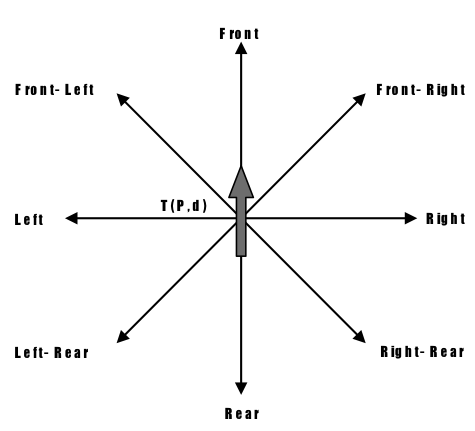
\includegraphics[width=0.3\textwidth, height=5cm]{2.RelatedWorks/fig2-b.png} \label{fig:img2-b} }
	\subfloat[]{ 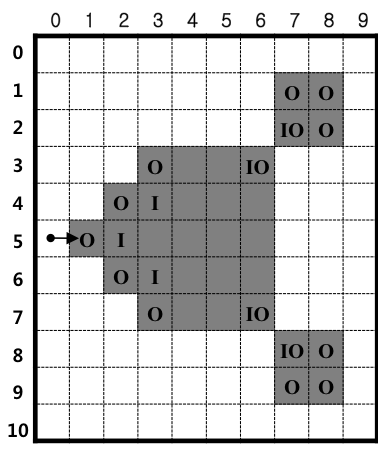
\includegraphics[width=0.3\textwidth, height=5cm]{2.RelatedWorks/fig2-c.png} \label{fig:img2-c} }
	 
	\caption{Directions and types of contour pixels. \protect\subref{fig:img2-a} Absolute direction $d$ \protect\subref{fig:img2-b} Relative direction $r$ \protect\subref{fig:img2-c} Types of contour pixels}
	\label{fig:image2}
\end{figure}


\subsubsection{Simple Boundary Follower}

SBF is also known as Papert's turtle algorithm \cite{Das1990Bivariate} and as square tracing algorithm\cite{Toussaint????Grids}, and it is the simplest contour tracing algorithm. Initially, the location of tracer $S$ is saved, and the tracer moves leftward or rightward; if the pixel tracer is located on a contour pixel, the tracer moves leftward, otherwise it moves rightward. The procedure is as given below.

\begin{algorithm}
	\caption{Algorithm of Simple Boundary Follower}\label{alg:sbf}
	\begin{algorithmic}[1]
	\Procedure{SBF}{}
	\State $\textit{T(P,d)} \gets \textit{S(P,d)}$
	\Do
	\If {$\textit{P}$ = black}
	\State $\textit{T(P,d)} \gets \textit{T(P}_{Left},\textit{d}_{Left} )  $
	\Else
	\State $\textit{T(P,d)} \gets \textit{T(P}_{Right},\textit{d}_{Right})$
	\EndIf
	\doWhile {$ \textit{T(P,d)}  \neq \textit{S(P,d)}$}
	\EndProcedure
	\end{algorithmic}
\end{algorithm}

\subsubsection{Modified Simple Boundary Follower}

SBF cannot trace an inner-outer corner pixel that is located at the left-rear. MSBF \cite{Gose1996Pattern} was invented to trace these pixels. If the tracer is adjacent to the left-rear inner-outer corner, this condition implies that its left-rear pixel is black (object) and the left and rear pixels are white (background); the tracer will move to the left-rear pixel and its direction is then changed toward the rear direction. After the movement, the tracer goes directly to the left pixel to avoid an infinite loop. Figure \ref{fig:image3} shows examples of the SBF and MSBF paths for a left-rear direction inner-outer corner. In the case of the SBF, if the tracer is on pixel $A$ with direction $N$, it misses pixel $B$. On the contrary, the MSBF can detour pixel $B$.

%%% Image 3
\begin{figure}[htbp]
	\centering
	\subfloat[]{ 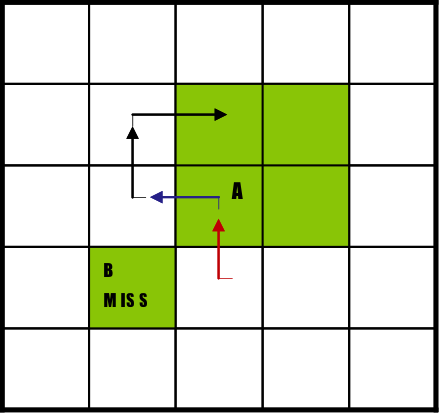
\includegraphics[width=0.25\textwidth]{2.RelatedWorks/fig3-a.png} \label{fig:img3-a} }
	\subfloat[]{ 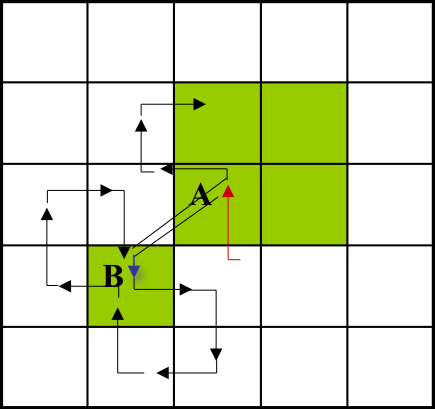
\includegraphics[width=0.25\textwidth]{2.RelatedWorks/fig3-b.png} \label{fig:img3-b} }
	 
	\caption{Detour of inner-outer corner at left-rear pixel (modified version of \cite{Gose1996Pattern}). \protect\subref{fig:img3-a} SBF \protect\subref{fig:img3-b} MSBF}
	\label{fig:image3}
\end{figure}

\subsubsection{Improved Simple Boundary Follower}

The SBF and MSBF require movement operations for both contour and background pixels; therefore, they waste time during movement on the background pixel and they cannot trace the inner corner pixel in front of the tracer \cite{Cheong2006Improved,Toussaint????Grids}. Hence, the ISBF \cite{Cheong2006Improved} is proposed based on our previous research for overcoming these limitations. The ISBF has six cases for following contour pixels based on the local patterns of the contour pixels. The modified version of \cite{Cheong2006Advanced} is as follows: 

\begin{algorithm}
	\caption{Algorithm of Improved Simple Boundary Follower}\label{alg:isbf}
	\begin{algorithmic}[1]
	\Procedure{ISBF}{}
	\State $\textit{T(P,d)} \gets \textit{S(P,d)}$, where \textit{P} is on black
	\Do
	\If {$\textit{P}_{Left}$ = black}
		\State $\textit{T(P,d)} \gets \textit{T(P}_{Left},\textit{d}_{Left} )  $
	\Else
		\If {$\textit{P}_{Left-Rear}$ = black and $\textit{P}_{Rear}$ = white}
			\State $\textit{T(P,d)} \gets \textit{T(P}_{Left-Rear},\textit{d}_{Rear} )  $
		\Else
			\If {$\textit{P}_{Front-Left}$ = black}
				\If {$\textit{P}_{Front}$ = black}
					\State $\textit{T(P,d)} \gets \textit{T(P}_{Front},\textit{d} )  $ and $\textit{T(P,d)} \gets \textit{T(P}_{Left}, \textit{d})$
				\Else
					\State $\textit{T(P,d)} \gets \textit{T(P}_{Front-Left},\textit{d} )  $
				\EndIf
			\ElsIf {$\textit{P}_{Front}$ = black}
				\State $\textit{T(P,d)} \gets \textit{T(P}_{Front},\textit{d}_{Right} )  $
			\Else
				\State $\textit{T(P,d)} \gets \textit{T(P},\textit{d}_{Rear} )  $
			\EndIf
		\EndIf
	\EndIf
	\doWhile {$ \textit{T(P,d)}  \neq \textit{S(P,d)}$}
	\EndProcedure
	\end{algorithmic}
\end{algorithm}

Figure \ref{fig:isbf} represents the tracing path of the ISBF based on the local contour patterns. While the SBF cannot trace in cases \ref{fig:img4-b} and \ref{fig:img4-d}, and the MSBF cannot follow in case \ref{fig:img4-d}, the ISBF successfully traces in all the cases. In the figure, the way point (dotted line) is subjected to a detection operation for determining whether it is black or white without employing a movement operation.

%%% Image 4
\begin{figure}[htbp]
	\centering
	\subfloat[]{ 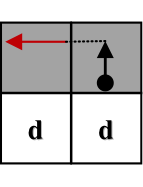
\includegraphics[height=2cm]{2.RelatedWorks/fig4-a.png} \label{fig:img4-a} }
	\subfloat[]{ 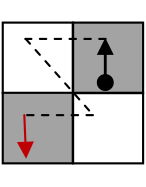
\includegraphics[height=2cm]{2.RelatedWorks/fig4-b.png} \label{fig:img4-b} }
	\subfloat[]{ 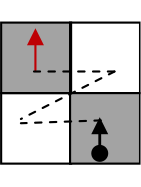
\includegraphics[height=2cm]{2.RelatedWorks/fig4-c.png} \label{fig:img4-c} }
	\subfloat[]{ 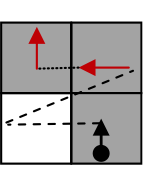
\includegraphics[height=2cm]{2.RelatedWorks/fig4-d.png} \label{fig:img4-d} }
	\subfloat[]{ 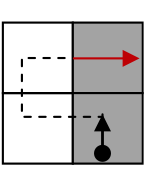
\includegraphics[height=2cm]{2.RelatedWorks/fig4-e.png} \label{fig:img4-e} }
	\subfloat[]{ 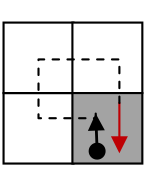
\includegraphics[height=2cm]{2.RelatedWorks/fig4-f.png} \label{fig:img4-f} }
	\subfloat[]{ 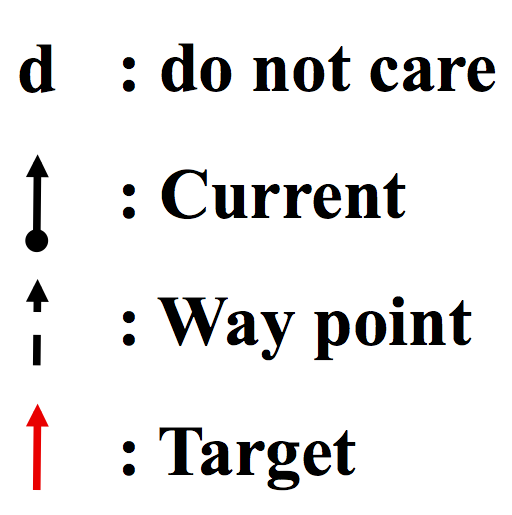
\includegraphics[height=2cm]{2.RelatedWorks/fig4-g.png} \label{fig:img4-g} }
	 
	\caption{Contour cases of ISBF \cite{Cheong2006Advanced} \protect\subref{fig:img4-a} Left neighbor \protect\subref{fig:img4-b} Innerouter corner at left-rear \protect\subref{fig:img4-c} Innerouter corner at front-left \protect\subref{fig:img4-d} Inner corner at front \protect\subref{fig:img4-e} Front neighbor \protect\subref{fig:img4-f} Outer corner}
	\label{fig:isbf}
\end{figure}

\subsubsection{Moore-Neighbor Tracing}
MNT (see, figure \ref{fig:img5-a}) finds the next contour pixel using 8 connected chain codes using a clockwise sequence starting from the rear pixel of the tracer, i.e., the tracer first moves toward the rear ($T (P_{Rear}, d_{Rear}))$ and finds the next clockwise contour pixel such as the left-rear, left, font-left, front, front-right, right, and right-rear pixels \cite{Toussaint????Grids}. 

\subsubsection{Modified Moore-Neighbor Tracing}
\textcolor{red}{To be written}

\subsubsection{Radial Sweep Algorithm}
RSA \cite{Mirante1982Radial} is similar to MNT, but its tracer has no directional information. Therefore, it maintains two points, namely, previous pixel and current pixel for the initial tracing direction. Figure \ref{fig:img5-b} illustrates an example of a tracing path by using RSA from $P_i$ to $P_{i+2}$. In the figure, the direction vector from $P_i$ to $P_{i-1}$ is first generated, and then the tracer searches for the next contour pixel using the previous pixel $P_{i-1}$ for the clockwise direction of the vector.

%%% Image 5
\begin{figure}[htbp]
	\centering
	\subfloat[]{ 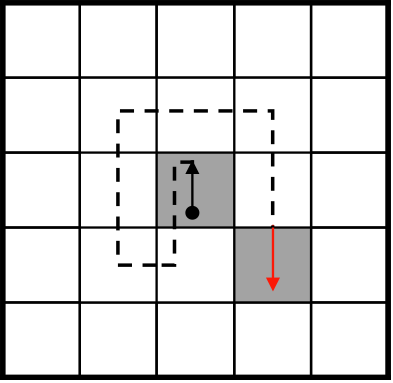
\includegraphics[width=0.3\textwidth]{2.RelatedWorks/fig5-a.png} \label{fig:img5-a} }
	\subfloat[]{ 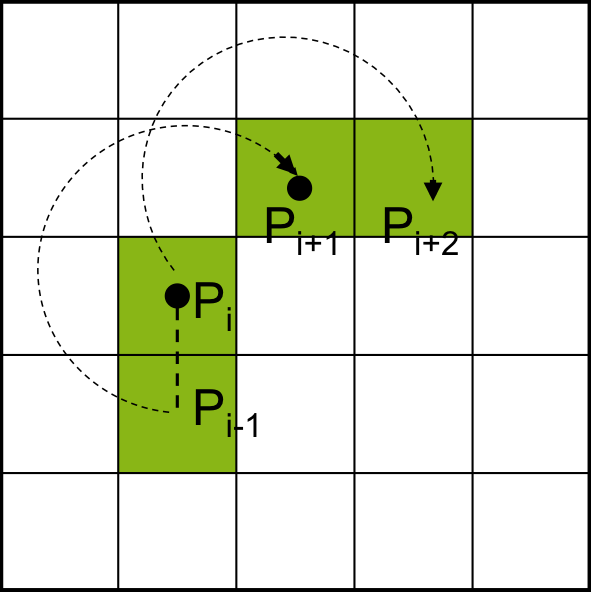
\includegraphics[width=0.3\textwidth]{2.RelatedWorks/fig5-b.png} \label{fig:img5-b} }
	\caption{Contour following sequence of MNT and RSA \protect\subref{fig:img5-a} MNT \protect\subref{fig:img5-b} RSA}
	\label{fig:mnt_rsa}
\end{figure}

\subsubsection{Theo Pavlidis Algorithm}
TPA \cite{Pavlidis2012Algorithms} considers only three adjacent pixels, e.g., front-left, front, and front-right for determining the next contour pixel. If all the three pixels are white, the tracer turns right. Figure \ref{fig:tpa} describes its sequence. 

%%% Image 6
\begin{figure}[htbp]
	\centering
	\subfloat[]{ 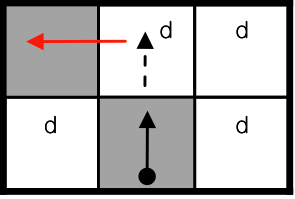
\includegraphics[width=0.25\textwidth]{2.RelatedWorks/fig6-a.png} \label{fig:img6-a} }
	\subfloat[]{ 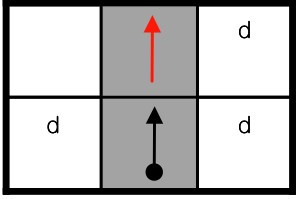
\includegraphics[width=0.25\textwidth]{2.RelatedWorks/fig6-b.png} \label{fig:img6-b} }
	\subfloat[]{ 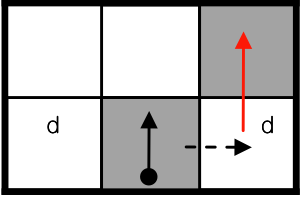
\includegraphics[width=0.25\textwidth]{2.RelatedWorks/fig6-c.png} \label{fig:img6-c} }
	\subfloat[]{ 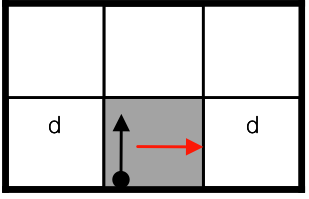
\includegraphics[width=0.25\textwidth]{2.RelatedWorks/fig6-d.png} \label{fig:img6-d} }
	 
	\caption{Contour following sequence of TPA\cite{Cheong2006Advanced}. \protect\subref{fig:img6-a} Front-Left contour \protect\subref{fig:img6-b} Front contour \protect\subref{fig:img6-c} Front-Right contour \protect\subref{fig:img6-d} Rotation}
	\label{fig:tpa}
\end{figure}

%%%%%%%%%%%%%%%%%%%%%%%%%%%%%
\subsection{Conventional Data Compression and Restoration}
The RD code method \cite{Miyatake1997Contour} comprises two major techniques. One traces the contour on the basis of the hybrid method using vertex following with run data and generates the corresponding RD codes. The other generates compressed contour data that can be used to restore the contour on the basis of representative points and their corresponding RD codes. The representative points are selected from the vertices of contour pixels and they are feature points of the contour. Moreover, the RD code can represent 10 local contour patterns and their corresponding following paths. Therefore, saving the representative points and their corresponding RD codes rather than all the contour points can reduce the memory size used to store the contour data. Figure \ref{fig:img7-a} \cite{Miyatake1997Contour} gives an example of representative points. The representative points in the RD method are of four types, namely, two outer corner points and two inner corner points, as shown in figure \ref{fig:img7-b}. Although this technique can save data in small files; it does not consider the inner-outer corner pixel. 

%%% Image 7
\begin{figure}[htbp]
	\centering
	\subfloat[]{ 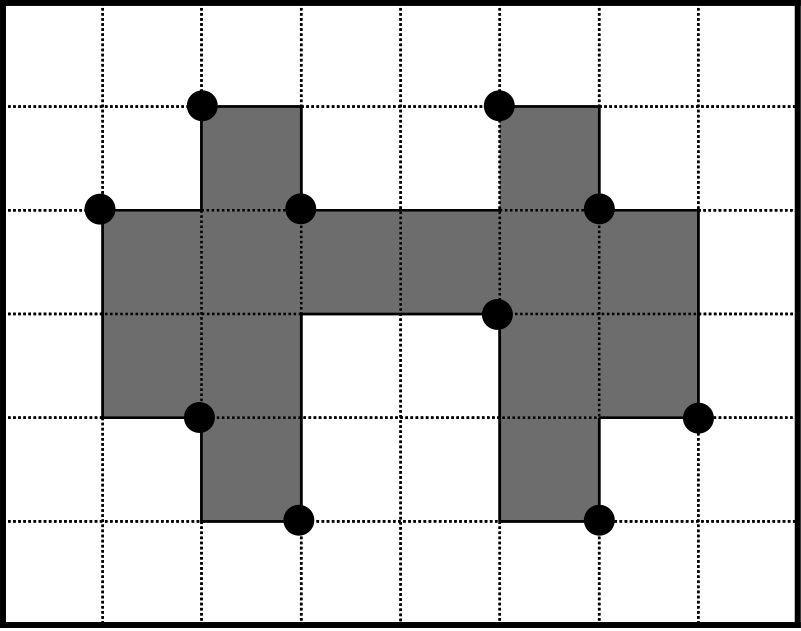
\includegraphics[height=4.5cm]{2.RelatedWorks/fig7-a.png} \label{fig:img7-a} }
	\subfloat[]{ 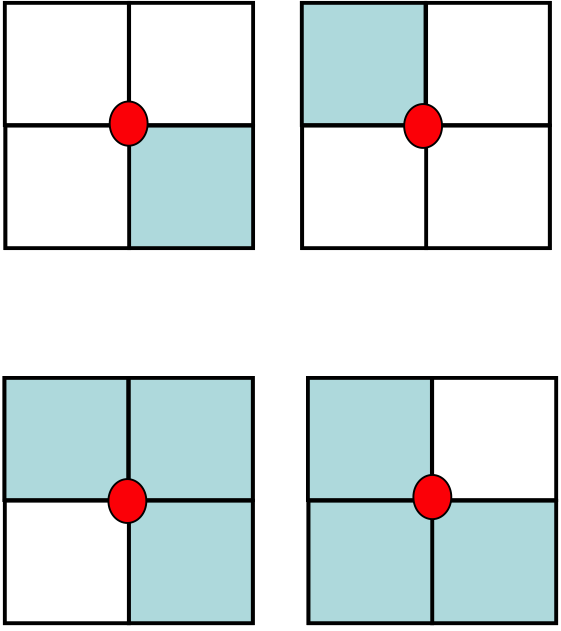
\includegraphics[height=4.5cm]{2.RelatedWorks/fig7-b.png} \label{fig:img7-b} }
	\caption{Representative points for data compression. \protect\subref{fig:img7-a} Representative points \cite{Miyatake1997Contour} \protect\subref{fig:img7-b} Cases of representative points}
	\label{fig:rdcode}
\end{figure}
%!TEX root = ../Fast_Contour_Tracing_Algorithm.tex
% -*- root: ../Fast_Contour_Tracing_Algorithm.tex -*-

\section{Analysis of Conventional Contour-following Algorithms}

% Figure \ref{fig:image8} illustrates the tracing results of pixel following methods based on the contour shown in figure \ref{fig:image1}. In the figure, the arrow with an anchor is the tracer at the starting pixel, a solid arrow shows the movement operation of the tracer, and a dotted line is the way point (detected pixel) for determining whether or not the pixel is a contour pixel for pixel following.

Figure \ref{fig:image8} illustrates the tracing results of the pixel-following methods based on the contour shown in Figure \ref{fig:image1}. In the figure, the arrow with an anchor is the tracer at the starting pixel, the solid arrow shows the movement operation of the tracer, and the dotted line is the way point (detected pixel) for determining whether or not the pixel is a contour pixel for pixel following.

%%% Image 8
\begin{figure}[htbp]
	\centering
	\subfloat[]{ 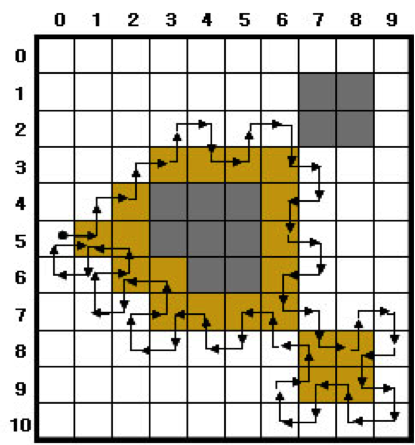
\includegraphics[width=0.33\textwidth]{3.Analysis/fig8-a.png} \label{fig:img8-a} }
	\subfloat[]{ 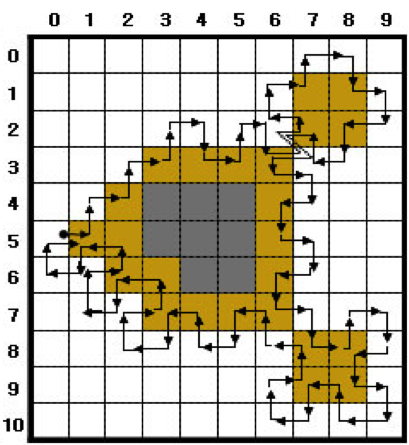
\includegraphics[width=0.33\textwidth]{3.Analysis/fig8-b.png} \label{fig:img8-b} }
	\subfloat[]{ 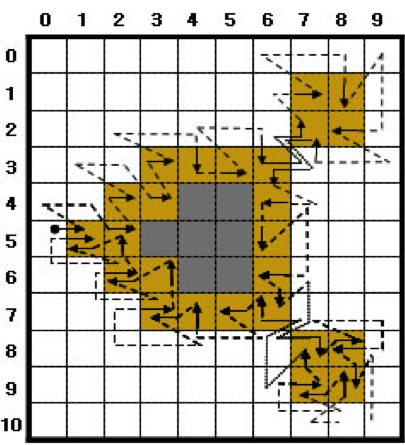
\includegraphics[width=0.33\textwidth]{3.Analysis/fig8-c.png} \label{fig:img8-c} } \\
	\subfloat[]{ 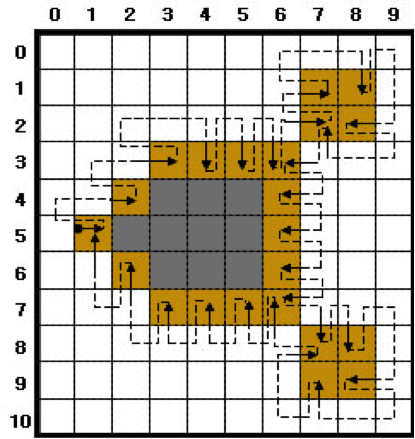
\includegraphics[width=0.33\textwidth]{3.Analysis/fig8-d.png} \label{fig:img8-d} }
	\subfloat[]{ 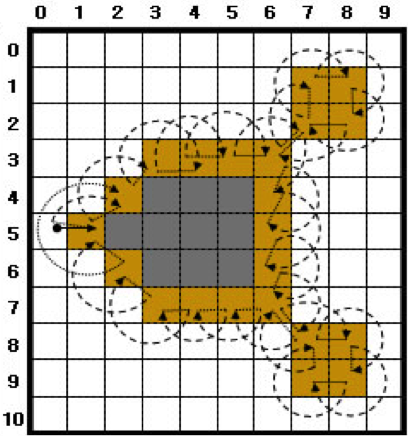
\includegraphics[width=0.33\textwidth]{3.Analysis/fig8-e.png} \label{fig:img8-e} }
	\subfloat[]{ 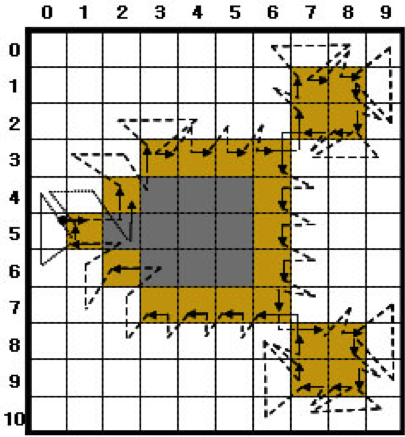
\includegraphics[width=0.33\textwidth]{3.Analysis/fig8-f.png} \label{fig:img8-f} }
	 
	\caption{Comparison of conventional contour pixel-following algorithms \protect\subref{fig:img8-a} SBF \protect\subref{fig:img8-b} MSBF \protect\subref{fig:img8-c} ISBF \protect\subref{fig:img8-d} MNT \protect\subref{fig:img8-e} RSA \protect\subref{fig:img8-f} TPA}
	\label{fig:image8}
\end{figure}

%%%%%
\subsection{Pixel-following Cases}

% As shown in figure \ref{fig:image8}, the ISBF traces most types of contour pixels such as the inner corner, outer corner, inner-outer corner, and straight-line pixels. In the case of the SBF, there are inconsistencies regarding tracing at the inner corner and inner-outer corner. For example, in the figure, the inner corner pixel (3, 6) and inner-outer corner pixel (7, 8) are traced, but the inner corner (3, 4) and inner-outer corner (7, 9) pixels are missed. In the case of the MSBF, all the inner-outer corner pixels are traced, but it has inconsistencies with regard to tracing the inner corner pixel. Moreover, the MNT, RSA, and TPA have no inconsistency problems but they cannot trace the inner corners. Among these algorithms, the TPA can be easily changed to trace an inner corner pixel since it has way points on the inner corners, as shown in figure \ref{fig:img8-f}. 

As shown in Figure \ref{fig:image8}, the ISBF traces most types of contour pixels such as the inner corner, outer corner, inner-outer corner, and straight-line pixels. In the case of the SBF, there are inconsistencies regarding tracing at the inner corner and inner-outer corner. For example, in the figure, the inner-corner pixel $(3, 6)$ and inner-outer corner pixel $(7, 8)$ are traced, but the inner corner $(3, 4)$ and inner-outer corner $(7, 9)$ pixels are missed. In the case of the MSBF, all the inner-outer corner pixels are traced, but it has inconsistencies with regard to tracing the inner-corner pixel. Moreover, the MNT, RSA, and TPA have no problems with consistency, but they cannot trace the inner corners. Among these algorithms, the TPA can be easily changed to trace an inner-corner pixel because it has waypoints on the inner corners, as shown in Figure \ref{fig:img8-f}.



%%%%%
\subsection{Start-up Condition and Stopping Criteria}

% The pixel following algorithm functions under the criteria of start and stop to avoid incompleteness of tracing and infinite tracing.
The pixel-following algorithm requires start- and stop-criteria to avoid incomplete or infinite contour trcing.

\subsubsection{Assumption for Start}

% Commonly, start of tracing occurs when the tracer enters a black pixel from a white pixel. Due to this reason, at the start of tracing, the tracer must be placed on a black pixel and its rear pixel $P_{Rear}$ should be white. Moreover, in the case of the MSBF and ISBF, if the $P_{Left-Rear}$ of the start pixel is an inner-outer corner pixel, they cannot trace all the contour pixels by using their stopping criteria \cite{Cheong2012Advanced}. In addition, TPA has to select a start pixel that has white pixels at the tracer positions $P_{Left}$, $P_{Left-Rear}$, and $P_{Right-Rear}$\cite{Ghuneim2015Contour}; otherwise, it cannot trace the left pixel of the contour. 

Commonly, tracing starts when the tracer enters a black pixel from a white pixel. Therefore, at the start of tracing, the tracer must be placed on a black pixel and its rear pixel $P_{Rear}$ should be white. Moreover, in the case of the MSBF and ISBF, if the $P_{Left-Rear}$ of the start pixel is an inner-outer corner pixel, it cannot trace all of the contour pixels using their stopping criteria\cite{Reddy2012Evaluation,Cheong2012Advanced}. In addition, TPA has to select a start pixel that has white pixels at the tracer positions $P_{Left}$, $P_{Left-Rear}$, and $P_{Right-Rear}$ \cite{Ghuneim2015Contour}; otherwise, it cannot trace the left pixel of the contour. 

\subsubsection{Stop Criterion}
% There are three methods for stopping the contour tracing \cite{Ghuneim2015Contour}. The first method is Jacob's stopping criterion \cite{Ghuneim2015Contour} that terminates the trace when the tracer reenters the start pixel with an absolute direction that is the same as the start direction, i.e., if the current tracer $T(P,d)$ is the same as the start tracer $S(P,d)$, the pixel following is terminated. The SBF, MSBF, and ISBF use this criterion and their tracing terminates at the start pixel, as shown in figures \ref{fig:img8-a}-\ref{fig:img8-c}. The second method uses the number of reentries to the start pixel. In figures \ref{fig:img8-d} and \ref{fig:img8-f}, the tracers of MNT and TPA revisit the start pixel (1, 5) with different directional information; therefore, they do not stop but go to the next contour pixel if the first method is applied. For this reason, if a specified number of reentries such as three or four times is satisfied, the trace is terminated \cite{Ghuneim2015Contour}. Sometimes, this method is not efficient because it requires unnecessary tracing to be performed one or more times. The final method checks the trace route that is traced by the previous pixel and current pixel of the tracer and determines whether or not it has already been passed. This method is used for RSA \cite{Ghuneim2015Contour,Mirante1982Radial} since its tracer has no directional information but only pixel location information. In other words, whenever the tracer enters the $i$-th contour pixel, the current pixel location $P_i$ is appended sequentially into the traced contour path. Moreover, if the traced path of $(P_{i-1}, P_i)$ appears twice, the tracing is terminated. This method can be applied for all pixel following methods and it is simpler than the second method; however, it requires more operations than Jacob's stopping criterion.

There are three methods for stopping the contour tracing \cite{Ghuneim2015Contour,Reddy2012Evaluation}. The first method is Jacob's stopping criterion \cite{Ghuneim2015Contour}, which terminates the trace when the tracer reenters the start pixel with an absolute direction that is the same as the start direction, i.e., if the current tracer $T(P,d)$ is the same as the start tracer $S(P,d)$, the pixel following is terminated. The SBF, MSBF, and ISBF use this criterion, and their tracing terminates at the start pixel, as shown in Figures \ref{fig:img8-a}-\ref{fig:img8-c}. The second method uses the number of reentries to the start pixel. In Figures \ref{fig:img8-d}-\ref{fig:img8-f}, the tracers of MNT and TPA revisit the start pixel $(1, 5)$ with different directional information; therefore, they do not stop, but rather go to the next contour pixel if the first method is applied. For this reason, if a specified number of reentries, e.g., three or four times, is satisfied, the trace is terminated \cite{Reddy2012Evaluation}. This method is sometimes not efficient because it requires unnecessary tracing to be performed one or more times. The final method checks the trace route that is traced by the previous pixel and current pixel of the tracer, and determines whether it has already been passed. This method is used for RSA \cite{Ghuneim2015Contour,Mirante1982Radial} because its tracer has only pixel-location information, and no directional information. In other words, whenever the tracer enters the $i$-th contour pixel, the current pixel location $P_i$ is appended sequentially into the traced contour path. Moreover, if the traced path of $(P_{i-1}, P_i)$ appears twice, the tracing is terminated. This method can be applied for all pixel-following methods, and it is simpler than the second method; however, it requires more operations than Jacob's stopping criterion.

\subsubsection{Limitations of Conventional Pixel-following Methods}

% The abovementioned conventional pixel following methods have certain limitations. First, some of the algorithms such as SBF and MSBF perform unnecessary movement operation on a white pixel, as shown in figures \ref{fig:img8-a} and \ref{fig:img8-b}. Second, all the algorithms cannot define the contour in the case of contour pixels; therefore, they cannot be a descriptive feature of the object and determine connectivity among objects. For example, in figure \ref{fig:img8-b}, the MSBF detects (2, 7) as the inner-outer corner pixel, but does not indicate (8, 7) as an inner-outer corner because the traced paths on the pixels are different. Moreover, the MSBF also cannot determine the inner corner, outer corner, and straight line pixel like the SBF does. In case of the ISBF, it determines the inner-outer corner, front inner corner, and front straight line pixels but cannot determine the left inner corner, left straight line and some of the outer corner pixels, as shown in figure \ref{fig:img8-c}. Similarly, MNT and RSA cannot determine and detect the inner corners, and TPA cannot classify the contour pixels into the different types of contour pixels. Finally, the data size of the traced contour must be considered. The pixel following methods save all the pixel points; therefore, their data are larger than those of the RD code method.

The abovementioned conventional pixel-following methods have certain limitations. First, some of the algorithms, such as SBF and MSBF, perform unnecessary movement operations on white pixels, as shown in Figures \ref{fig:img8-a} and \ref{fig:img8-b}. Second, not all of the algorithms can define the contour in the case of contour pixels; therefore, they cannot be a descriptive feature of the object and determine connectivity among objects. For example, in Figure \ref{fig:img8-b}, the MSBF detects $(2, 7)$ as the inner-outer corner pixel, but does not indicate $(8, 7)$ as an inner-outer corner because the traced paths on the pixels are different. Moreover, the MSBF also cannot determine the inner corner, outer corner, and straight-line pixel, as is the case with the SBF. In the case of the ISBF, it determines the inner-outer corner, front-inner corner, and front-straight line pixels, but cannot determine the left-inner corner, left-straight line, and some of the outer-corner pixels, as shown in Figure \ref{fig:img8-c}. Similarly, MNT and RSA cannot determine and detect the inner corners, and TPA cannot classify the contour pixels into the different types of contour pixels. Finally, the data size of the traced contour must be considered. The pixel-following methods save all the pixel points; therefore, their data are larger than those of the RD code method.



%!TEX root = ../Fast_Contour_Tracing_Algorithm.tex
% -*- root: ../Fast_Contour_Tracing_Algorithm.tex -*-

\section{Proposed Contour-tracing Algorithm}

% In this section, we propose a novel pixel following algorithm that traces contour pixels by considering their local patterns. Therefore, it can classify the contour pixel into contour types such as inner corner, outer corner, inner-outer corner, and straight line; further, it can easily determine the next contour pixel. Moreover, it can determine and save representative points of an image, like the RD code method, by using pixel following but not using run-data-based following. In addition, the data can be restored to the original contour pixels without the RD code data.

In this section, we propose a novel pixel-following algorithm that traces contour pixels by considering their local patterns. Therefore, it can classify the contour pixel as inner corner, outer corner, inner-outer corner, and straight-line contour types. Further, it can easily determine the next contour pixel. Moreover, it can determine and save representative points of an image, such as the RD code method, by using pixel following but not using run-data-based following. In addition, the data can be restored to the original contour pixels without the RD code data.

\subsection{Contour Following}

\subsubsection{Assumptions for Start-up and Stopping Criteria}

% The proposed algorithm runs under two assumptions for start. One is the general condition for pixel following: the rear pixel of the tracer on the start pixel is white. The other is that there is no left-rear inner-outer corner for the tracer at the start position, i.e., if the rear and the left pixels are white and the rear-left pixel is black, the start pixel has to be changed. These are the same starting conditions as those for the MSBF and ISBF. Moreover, the stop criteria of the proposed algorithm is Jacob's stopping criterion and the tracer is always on a contour pixel.

The proposed algorithm runs under two assumptions for starting. One is the general condition for pixel following, where the rear pixel of the tracer on the start pixel is white. The other is that there is no left-rear inner-outer corner for the tracer at the start position, i.e., if the rear and the left pixels are white and the rear-left pixel is black, the start pixel has to be changed. These are the same starting conditions as those used for the MSBF and ISBF. Moreover, the stop criteria of the proposed algorithm is Jacob’s stopping criterion, and the tracer is always on a contour pixel. 

\begin{figure}[htbp]
	\centering
	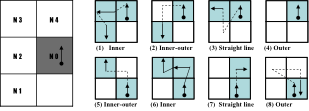
\includegraphics[width=1.0\textwidth]{4.Proposed/proposed_cases.png}
	\caption{Contour Tracing Cases for Proposed Contour-following Algorithm.}
	\label{fig:image9}
\end{figure}
\JHMEMO{Change the image 9}


\subsubsection{Procedures}

% The proposed algorithm has two stages. First, the tracer follows the contour pixel on the basis of the intensities of the left-rear and left pixels. After that, the tracer follows the contour pixels on the basis of the intensities of the front and front-left pixels. Figure \ref{fig:image9} shows the contour tracing cases of the proposed contour following algorithm. In the figure, the tracer is first on $N0$ queries states of $N1$ and $N2$, as shown in figure \ref{fig:image9} (a), and then the states determine the corresponding  path to trace among cases (1)-(4), as shown in figure \ref{fig:image9} (b). After stage 1, the moved tracer queries states N3 and N4 and then it traces contour pixels along the corresponding path using the states among cases (5)-(8). 

The proposed algorithm has two stages. First, the tracer follows the contour pixel based on the intensities of the left-rear and left pixels. After that, the tracer follows the contour pixels according to the intensities of the front and front-left pixels.  \ref{fig:image9} shows the contour tracing cases for the proposed contour-following algorithm. In the figure, the tracer is first on $N0$ queries states of $N1$ and $N2$, as shown in  \JHMEMO{\ref{fig:image9}(a)}, and then the states determine the corresponding path to be traced from among cases (1)–(4), as shown in Figure \JHMEMO{\ref{fig:image9}(b)}. After stage 1, the moved tracer queries states N3 and N4, and it then traces contour pixels along the corresponding path using the states from among cases (5)–(8). 

% Hence, by using the proposed algorithm, the inner corners are traced as case (1) or case (6), the inner-outer corners are traced as case (2) or case (5), the outer corners are determined as case (4) or case (8), and the straight-line pixels are determined as the other cases. Therefore, all the cases are easily classified by using the algorithm. 

Hence, by using the proposed algorithm, the inner corners traced are considered as case (1) or case (6), the inner-outer corners are considered as case (2) or case (5), the outer corners are considered as case (4) or case (8), and the straight-line pixels are considered as the other cases. Therefore, all the cases are easily classified using the algorithm. 




\subsubsection{States}

\begin{figure}[htbp]
	\centering
	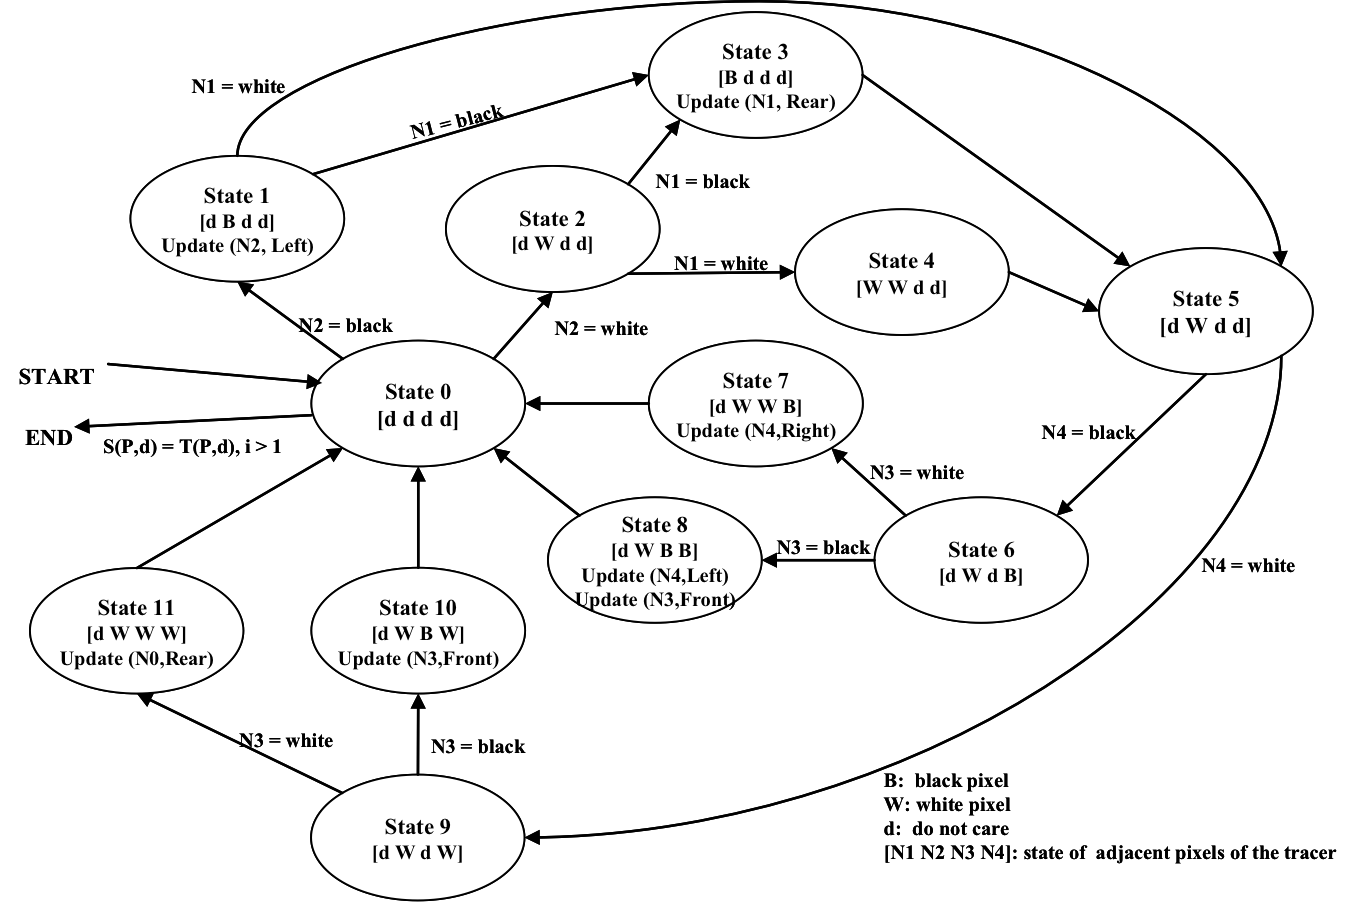
\includegraphics[width=1.0\textwidth]{4.Proposed/state.png}
	\caption{State Transition of Automation for Proposed Algorithm.}
	\label{fig:image10}
\end{figure}

% Figure \ref{fig:image10} describes the state transition for the automation of the proposed algorithm. In the figure, the start and termination occur at State 0; the first stage runs using States 1-4 and then it transits to State 5. The second stage continues from State 5 using States 6-11 and then it transits to State 0. For example, case (1) in figure \ref{fig:image9} can be executed by the transit sequence State 1, State 3, and State 5. 

\ref{fig:image10} describes the state transition for the automation of the proposed algorithm. In the figure, the start and termination occur at State 0. The first stage runs using States 1–4, and it then transits to State 5. The second stage continues from State 5 using States 6–11, and it then transits to State 0. For example, case (1) in Figure 9 can be executed using the transit sequence State 1, State 3, and State 5. 

% In figure \ref{fig:image10}, $[N1 N2 N3 N4]$ represents the intensity vector of the tracer's four adjacent pixels shown in figure \ref{fig:image9} (a). In the vector, $d$ implies ``do not care''; $B$, a contour pixel (black); and $W$, the background pixel (white). Moreover, Update $(P,d)$ refers to the movement operation where $P$ is the new contour pixel location and $d$ is the new directional information for the tracer. In State 1 and State 3, the updates occur based on the tracer of State 0, and other updates are based on the tracer information in State 5.

In \ref{fig:image10}, $[N1 N2 N3 N4]$ represents the intensity vector of the tracer’s four adjacent pixels shown in Figure \JHMEMO{\ref{fig:image9}(a)}. In the vector, $d$ implies ``do not care''; $B$ represents a contour pixel (black), and $W$ represents the background pixel (white). Moreover, Update $(P,d)$ refers to the movement operation where $P$ is the new contour-pixel location and $d$ is the new directional information for the tracer. In States 1 and 3, the updates occur based on the tracer of State 0, and other updates are based on the tracer information in State 5.

\subsubsection{Characteristics of Proposed Algorithm}

% We designed the proposed algorithm based on two stages with two major goals. First, the check operation for stopping occurs only at State 0; therefore, the number of checking operations on black pixels are reduced. In other words, the proposed algorithm examines that the check operation occurs when only the tracer has a white rear pixel. This is more efficient as compared to the check operation occuring for every contour pixel because its start condition and stop criterion also satisfy that the rear pixel of the tracer on the start pixel is white. Therefore, the transition of stage 2 to States 6 to 11 for processing cases (5) to (8) is designed such that it can be returned to State 0 only if the tracer has a white rear pixel, and it reduces any unnecessary operations for checking to stop. Besides, the tracers of cases (2) and (4) have a white rear pixel after movement but their end conditions are not considered. In case (2), at the start the tracer avoids the inner-outer corner pixels as the start and end pixel. Moreover, in case (4), the tracer has no update; therefore, it is unnecessary to perform check operation twice. 

We designed the proposed algorithm based on two stages with two major goals. First, the check operation for stopping occurs only at State 0; therefore, the number of checking operations on black pixels is reduced. In other words, the proposed algorithm verifies that the check operation occurs when only the tracer has a white rear pixel. This is more efficient when compared to the check operation that occurs for every contour pixel because its start condition and stop criterion also satisfy the condition that the rear pixel of the tracer on the start pixel should be white. Therefore, the transition of stage 2 to States 6–11 for processing cases (5) to (8) is designed such that it can be returned to State 0 only if the tracer has a white rear pixel, and it reduces any unnecessary operations that are required to stop the checking. Besides, the tracers of cases (2) and (4) have a white rear pixel after the movement, but their end conditions are not considered. In case (2), at the start, the tracer avoids the inner-outer corner pixels as the start and end pixel. Moreover, in case (4), the tracer has no update; therefore, it is unnecessary to perform the check operation twice. 

% Second, the proposed algorithm reduces some of the redundant operations used for detecting white pixels. The conventional algorithms do not consider white pixels in the previous path; therefore, they sometimes redetect white pixels on the previous tracing during the current tracing. For example, in figure 8, the white pixel at (4, 2) is detected twice while determining contour pixels such as (4, 3) and (5, 3). Moreover, RSA detects (4, 2) three time while determining (4, 3), (5, 3), and (6, 3). On the contrary, the proposed algorithm has two stages and its second stage avoids the previous path. \textcolor{red}{Figure 11} shows the contour tracing results for the proposed algorithm and it detects (4, 2) once for contour tracing. Moreover, the figure shows that the proposed algorithm has fewer operations on the white pixels as compared to conventional pixel following methods, as shown in figure \ref{fig:comparison}, and traces all the types of contours. 

Second, the proposed algorithm eliminates some of the redundant operations that are used to detect white pixels. The conventional algorithms do not consider white pixels in the previous path; therefore, they sometimes redetect white pixels on the previous tracing during the current tracing. For example, in Figure \ref{fig:comparison}, the white pixel at $(4, 2)$ is detected twice while determining contour pixels such as $(4, 3)$ and $(5, 3)$. Moreover, RSA detects $(4, 2)$ three times while determining $(4, 3)$, $(5, 3)$, and $(6, 3)$. On the contrary, the proposed algorithm has two stages, and its second stage avoids the previous path. Figure \textcolor{red}{Figure 11} shows the contour-tracing results obtained for the proposed algorithm, and it detects $(4, 2)$ once for contour tracing. Moreover, the figure shows that the proposed algorithm has fewer operations on the white pixels when compared to conventional pixel-following methods, as shown in Figure \ref{fig:comparison}, and it traces all types of contours. 

% The pseudo-code of the proposed algorithm is as below: 

The pseudocode of the proposed algorithm is given below: 

\begin{algorithm}
	\caption{Algorithm of Proposed Algorithm}
	\label{alg:proposed}
	\begin{algorithmic}[1]
	\Procedure{Proposed\_Tracer}{}
	\State $\textit{T(P,d)} \gets \textit{S(P,d)}$, where $P$ is on black, $P_{Rear}$ is on white and $i \gets 1$
	\LineComment{Whenever $T(P,d)$ is updated, $i$ increases $1$ and $T(p',d')$ is saved automatically}
	\Do
	\LineComment{State 1}
	\If {$\textit{P}_{Left-Rear}$ = black}
		\If {$\textit{P}_{Left}$ = black}
			\LineComment{Case 1}
			\State $\textit{T(P,d)} \gets \textit{T(P}_{Left},\textit{d}_{Left} )  $ and $\textit{Code(i)} \gets ``Inner''$ and $\textit{T(P,d)} \gets \textit{T(P}_{Left}, \textit{d}_{Left})$
		\Else
			\LineComment{Case 2}
			\State $\textit{Code(i)} \gets ``Inner-outer''$ and $\textit{T(P,d)} \gets \textit{T(P}_{Left-Rear},\textit{d}_{Rear} )  $
			\State $\textit{Code(i)} \gets ``Inner-outer''$
		\EndIf
	\Else
		\If {$\textit{P}_{Left}$ = black}
			\LineComment{Case 3}
			\State $\textit{T(P,d)} \gets \textit{T(P}_{Left},\textit{d}_{Left} )  $ and $\textit{Code(i)} \gets ``Straight''$
		\Else
			\LineComment{Case 4}
			\State $\textit{Code(i)} \gets ``Outer''$
		\EndIf
	\EndIf


	\LineComment{Stage 2}
	\If {$\textit{P}_{Front-Left}$ = black}
		\If {$\textit{P}_{Front}$ = black}
			\LineComment{Case 6}
			\State $\textit{T(P,d)} \gets \textit{T(P}_{Front},\textit{d}_{Left} )  $ and $\textit{Code(i)} \gets ``Inner''$ and $\textit{T(P,d)} \gets \textit{T(P}_{Front}, \textit{d}_{Right})$
		\Else
			\LineComment{Case 5}
			\State $\textit{Code(i)} \gets ``Inner-outer''$ and $\textit{T(P,d)} \gets \textit{T(P}_{Front-Left},\textit{d} )  $
			\State $\textit{Code(i)} \gets ``Inner-outer''$
		\EndIf
	\ElsIf {$\textit{P}_{Front}$ = black}
		\LineComment{Case 7}
		\State $\textit{T(P,d)} \gets \textit{T(P}_{Front},\textit{d}_{Right} )  $
	\Else
		\LineComment{Case 8}
		\State $\textit{T(P,d)} \gets \textit{T(P},\textit{d}_{Rear} )  $ and $i \gets i-1$ and $\textit{Code(i)} \gets ``Outer''$
	\EndIf


	\doWhile {$ \textit{T(P,d)}  \neq \textit{S(P,d)}$}
	\EndProcedure
	\end{algorithmic}
\end{algorithm}

% Table \ref{table:table2} describes the tracing results obtained by using the proposed algorithm up to the stage the tracer enters the 11th pixel. The code represents the contour pixel type and it is classified automatically during tracing. 

Table \ref{table:table2} describes the tracing results that were obtained by using the proposed algorithm up to the stage at which the tracer enters the 11th pixel. The code represents the contour pixel type, and it is classified automatically during tracing. 

\begin{table}[h]
	\centering
	\begin{tabularx}{0.7\textwidth}{Y|Y|Y|Y}
		\hline
		\multirow{2}{*}{$Sequence(i)$} &  \multicolumn{2}{|c|}{P}  & \multirow{2}{*}{$Code(i)$} \\
		\cline{2-3}
		             &$x$       & $y$ & \\
		\hline
		1 & 1 & 5 & Outer \\
		2 & 2 & 5 & Inner \\
		3 & 2 & 4 & Outer \\
		4 & 3 & 4 & Inner \\
		5 & 3 & 3 & Outer \\
		6 & 4 & 3 & Straight \\
		7 & 5 & 3 & Straight \\
		8 & 6 & 3 & Inner-outer \\
		9 & 7 & 2 & Inner-outer \\
		10 & 7 & 1 & Outer \\
		11 & 8 & 1 & \\

		\hline
	\end{tabularx}
	\caption{Result Table of the Proposed Contour Tracing}
	\label{table:table2}
\end{table}

% In the table, $Code (i)$ represents only one code, the contour pixel type, per contour pixel but it can have several codes, for example, there is an outer corner pixel and an inner-outer corner pixel. 

In the table, $Code (i)$ represents only one code, the contour pixel type per contour pixel, but it can have several codes. For example, there is an outer-corner pixel and an inner-outer corner pixel. 


%%%%%%%%%%%%%%%%%
 \subsection{Data Compression and Restoration}

 % The proposed algorithm saves representation points and the inner-outer corner points in the form of compressed data in order to reduce the data size. The representation points are feature points that are used for storing and restoring contour pixels, while the inner-outer corner points are used for accurately restoring the inner-outer corner pixels. 

 The proposed algorithm saves representation points and the inner-outer corner points in the form of compressed data in order to reduce the data size. The representation points are feature points that are used for storing and restoring contour pixels, while the inner-outer corner points are used for accurately restoring the inner-outer corner pixels. 

 \subsubsection{Data Structure}
 % The representative points and inner-outer corner points are represented as vertices of contour pixels. Figure \textcolor{red}{12 (a)} shows the point types of the proposed algorithm. The representative point is of seven types, namely, two outer corners, two inner corners, and one inner-outer corner. Moreover, the inner-outer corner point has two types. Figure \textcolor{red}{12 (b)} illustrates all cases of contour tracing for the proposed algorithm and their corresponding representative points and inner-outer corner points. 

 The representative points and inner-outer corner points are represented as vertices of contour pixels. Figure \JHMEMO{12(a)} shows the point types of the proposed algorithm. There are seven types of representative point. They are two outer corners, two inner corners, and one inner-outer corner. In addition, there are two types of inner-outer corner point. Figure \JHMEMO{12(b)} illustrates all cases of contour tracing for the proposed algorithm and their corresponding representative points and inner-outer corner points. 

 % These points are saved as a sequence during contour tracing. If an $i$-th representative point $R_i$ is equivalent to $(r_{i,x}, r_{i,y})$, then the set of representative points $R$ is given by $\{R_0, R_1, R_2, … , R_{n-1}\}$ and $R_0 = R_n$ because the starting and ending points are the same. Similarly, if $C_j$ is the $j$-th inner-outer corner point, it can be represented using its coordinate and its type. The type of the point $C_{j,T}$ is assigned to be NW-SE or NE-SW, as shown in figures \textcolor{red}{12 (a)}. Table \ref{table:data_structure} shows the data structure for data compression and restoration of the contour pixels by using the proposed algorithm. 

 These points are saved as a sequence during contour tracing. If the i-th representative point Ri is equivalent to $(r_{i,x}, r_{i,y})$, then the set of representative points $R$ is given by $\{R_0, R_1, R_2, … , R_{n-1}\}$ and $R_0 = R_n$ because the starting and ending points are the same. Similarly, if $C_j$ is the $j$-th inner-outer corner point, it can be represented using its coordinate and its type. The type of point $C_{j,T}$ is assigned to be $NW-SE$ or $NE-SW$, as shown in Figure \JHMEMO{12(a)}. Table \ref{table:data_structure} shows the data structure for data compression and the restoration of the contour pixels using the proposed algorithm. 

 %%% Image 11
\begin{figure}[htbp]
	\centering
	\subfloat[]{ 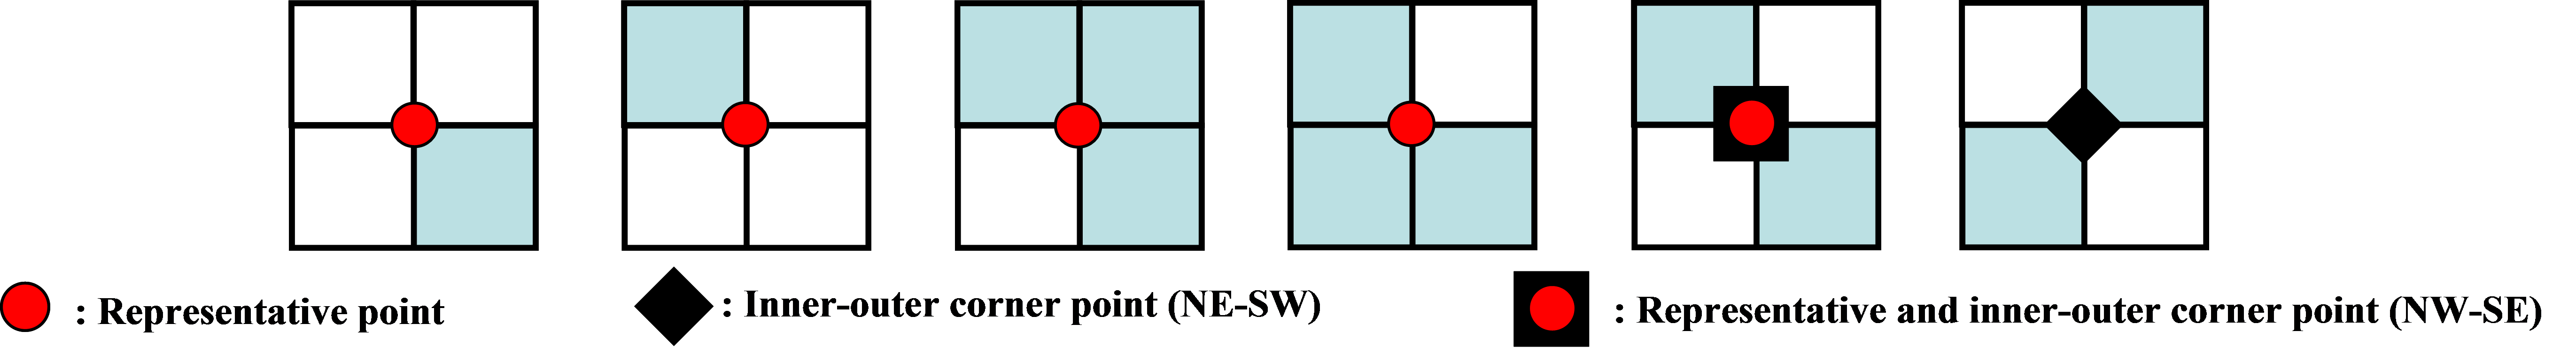
\includegraphics[width=1.0\textwidth]{4.Proposed/fig11-a.png} \label{fig:img11-a} } \\
	\subfloat[]{ 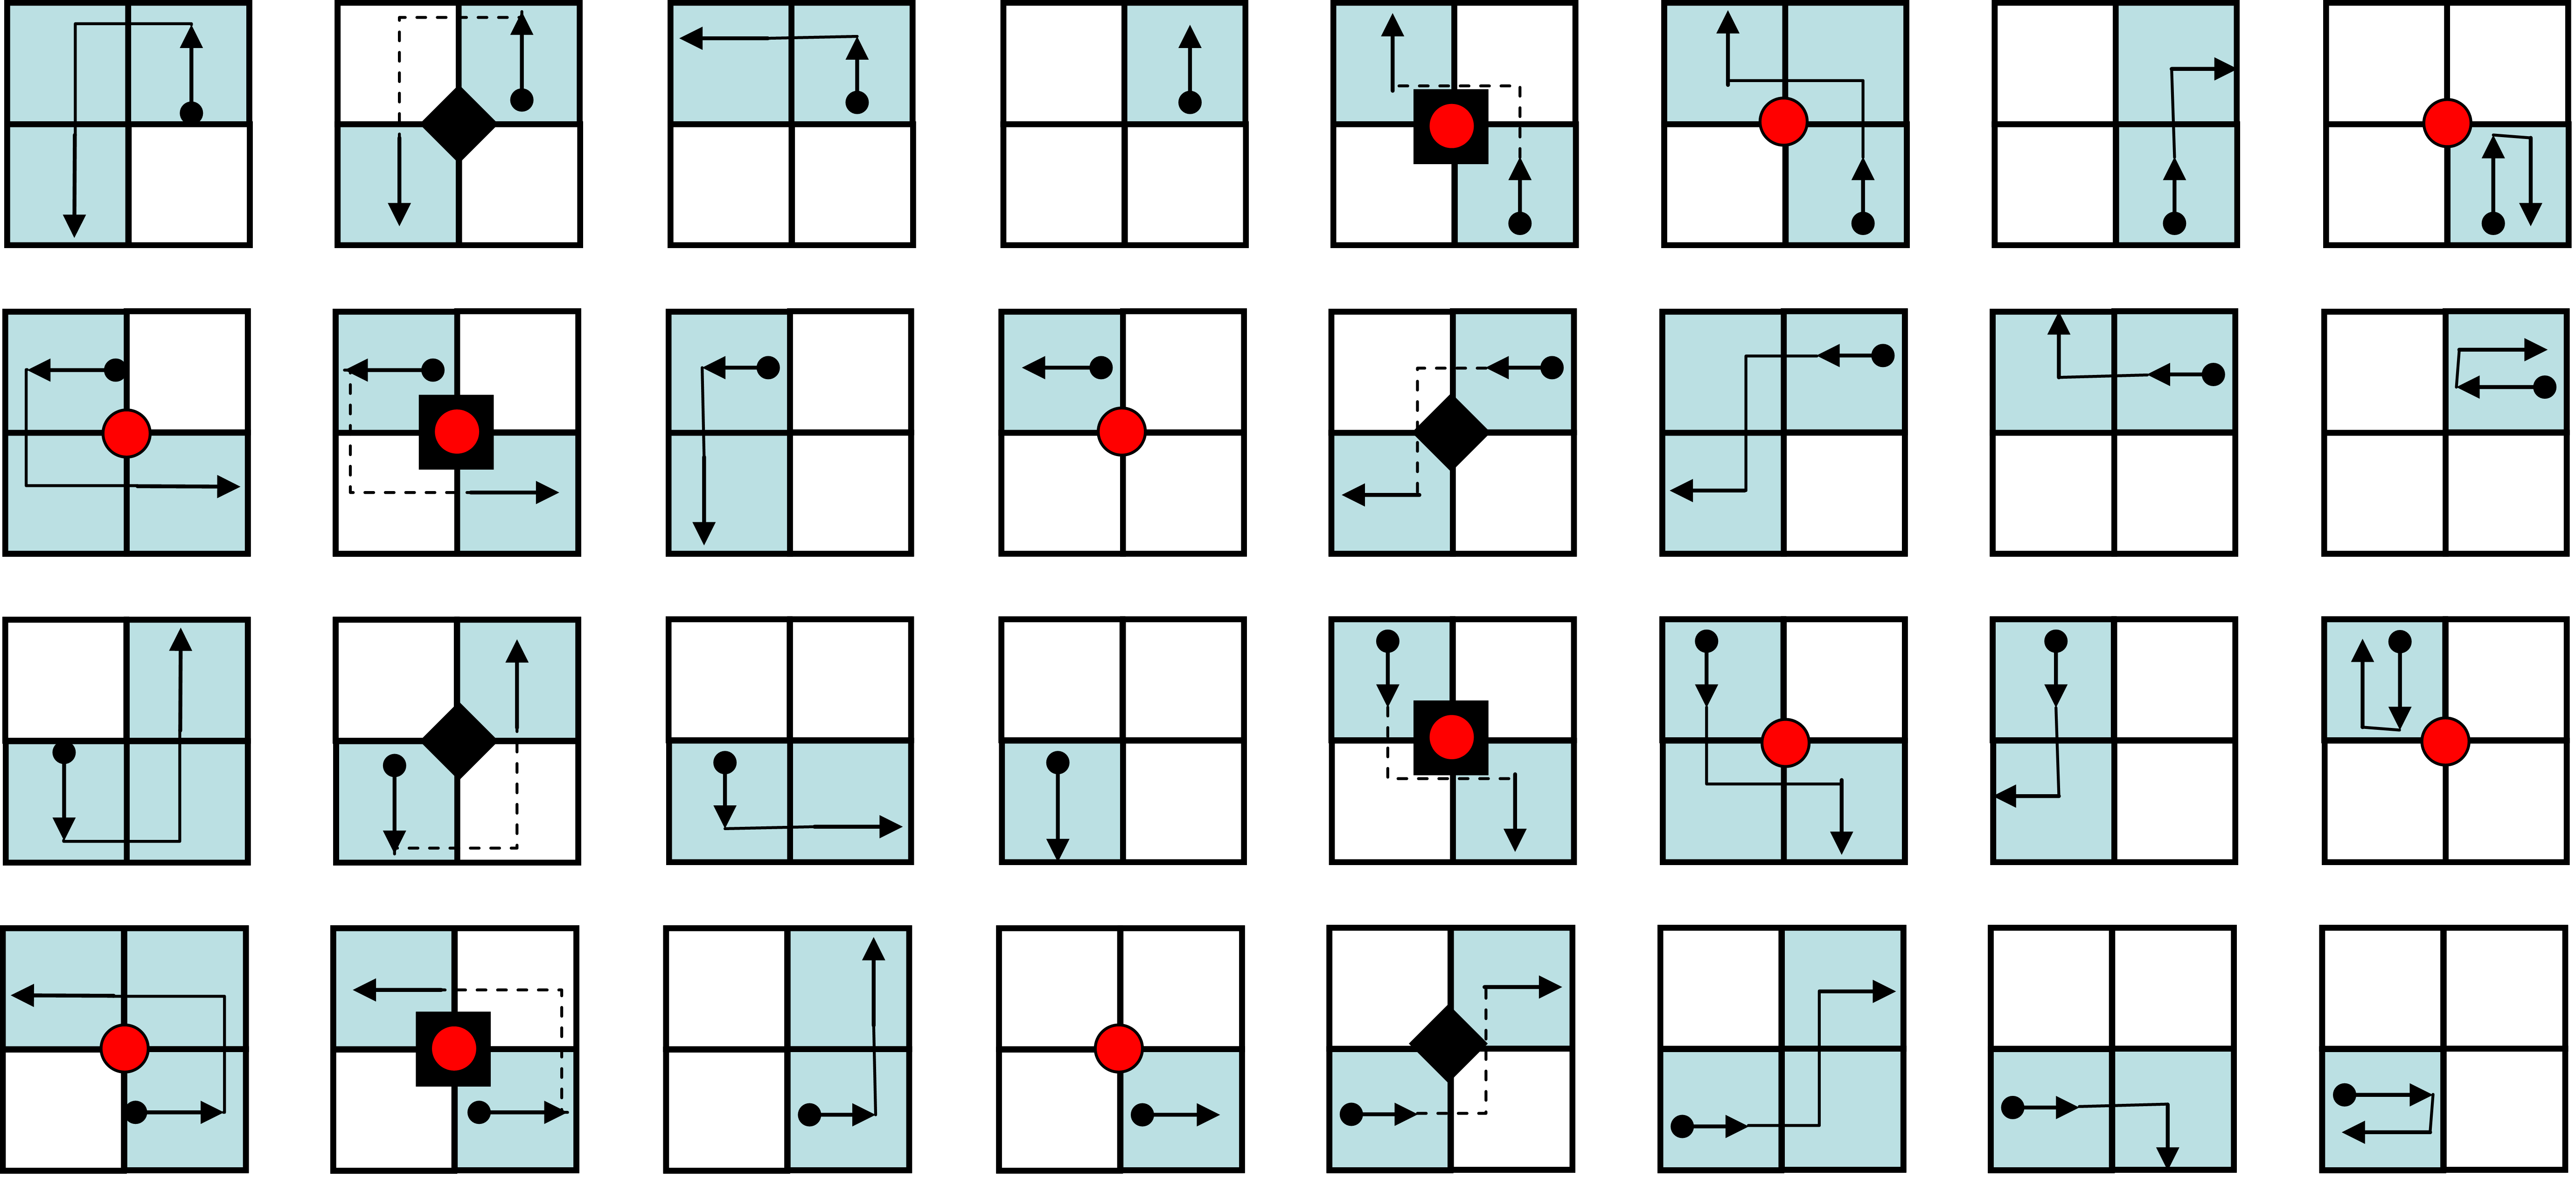
\includegraphics[width=1.0\textwidth]{4.Proposed/fig11-b.png} \label{fig:img11-b} }
	\caption{Contour Pixel Reconstruction. \protect\subref{fig:img11-a} Representative points and inner-outer corner points \protect\subref{fig:img11-b} Cases of the proposed algorithm }
	\label{fig:image11}
\end{figure}


 \begin{table}[h]
	\centering
	\begin{tabularx}{0.7\textwidth}{YYYYY}
		\hline
		\multicolumn{2}{c}{Representative Points($R_i$)} & 
		\multicolumn{3}{c}{Inner-outer Corner($C_i$)} \\
		\hline
		$x$ & $y$ & $x$ & $y$ & Type \\
		\hline

		$r_{1,x}$ & $r_{1,y}$ & $C_{1,x}$ & $C_{1,y}$ & $C_{1,T}$ \\
		$r_{2,x}$ & $r_{2,y}$ & $C_{2,x}$ & $C_{2,y}$ & $C_{2,T}$ \\
		... & ... & ... & ... & ...\\
		\hline
	\end{tabularx}
	\caption{Data Structure of Proposed Contour Tracer.}
	\label{table:data_structure}
\end{table}

\subsubsection{Contour Pixel Restoration}

% For restoration, we proposed a restoration algorithm comprising two stages, namely, contour restoration and inner-outer corner restoration.

For the restoration, we proposed a restoration algorithm comprising two stages, namely, contour restoration and inner-outer corner restoration.

\subsubsection{Contour Restoration with Representation Points}

\textcolor{red}{Change the above title to subsubsubsection}

% The sequence of representative points is important information for reconstructing the contour pixels because it represents the contour tracing sequence. Hence, by using the sequence of representative points and the relative location between adjacent representative points in the representative point table, the contour can be restored easily. If there are two sequential representative points $R_i$ and $R_{i+1}$, $\Lambda(R_i, R_{i+1})$ as the relative position classifier from $R_i$ to $R_{i+1}$ can be described as 

The sequence of representative points is important for the reconstruction of the contour pixels because it represents the contour-tracing sequence. Hence, by using the sequence of representative points and the relative location between adjacent representative points in the representative point table, the contour can be restored easily. If there are two sequential representative points $R_i$ and $R_{i+1}$, $\Lambda(R_i, R_{i+1})$, which is the relative position classifier from $R_i$ to $R_{i+1}$, can be described as 

\begin{equation}
	\Lambda(R_i, R_{i+1}) = \begin{cases}
	NE\: \text{where\:} r_{i,x} < r_{i+1,x}\: \text{and\:} r_{i,y} > r_{i+1,y} \\ 
	SE\: \text{where\:} r_{i,x} < r_{i+1,x}\: \text{and\:} r_{i,y} < r_{i+1,y} \\ 
	NW\: \text{where\:} r_{i,x} > r_{i+1,x}\: \text{and\:} r_{i,y} > r_{i+1,y} \\ 
	SW\: \text{where\:} r_{i,x} > r_{i+1,x}\: \text{and\:} r_{i,y} < r_{i+1,y}
	\end{cases}
	\label{eq:lambda}
\end{equation}

% Figure \textcolor{red}{13} shows the contour pixel reconstruction methods using the relative positions from $R_i$ to $R_{i+1}$. In the case of SE or NW, the contour pixels are filled in a clockwise manner and in the other cases, these pixels are filled in a counterclockwise manner.
Figure \ref{fig:image12} shows the contour-pixel reconstruction methods using the relative positions from $R_i$ to $R_{i+1}$. In the case of $SE$ or $NW$, the contour pixels are filled in a clockwise manner, while in the other cases, these pixels are filled in a counterclockwise manner.

%%% Image 12
\begin{figure}[htbp]
	\centering
	\subfloat[]{ 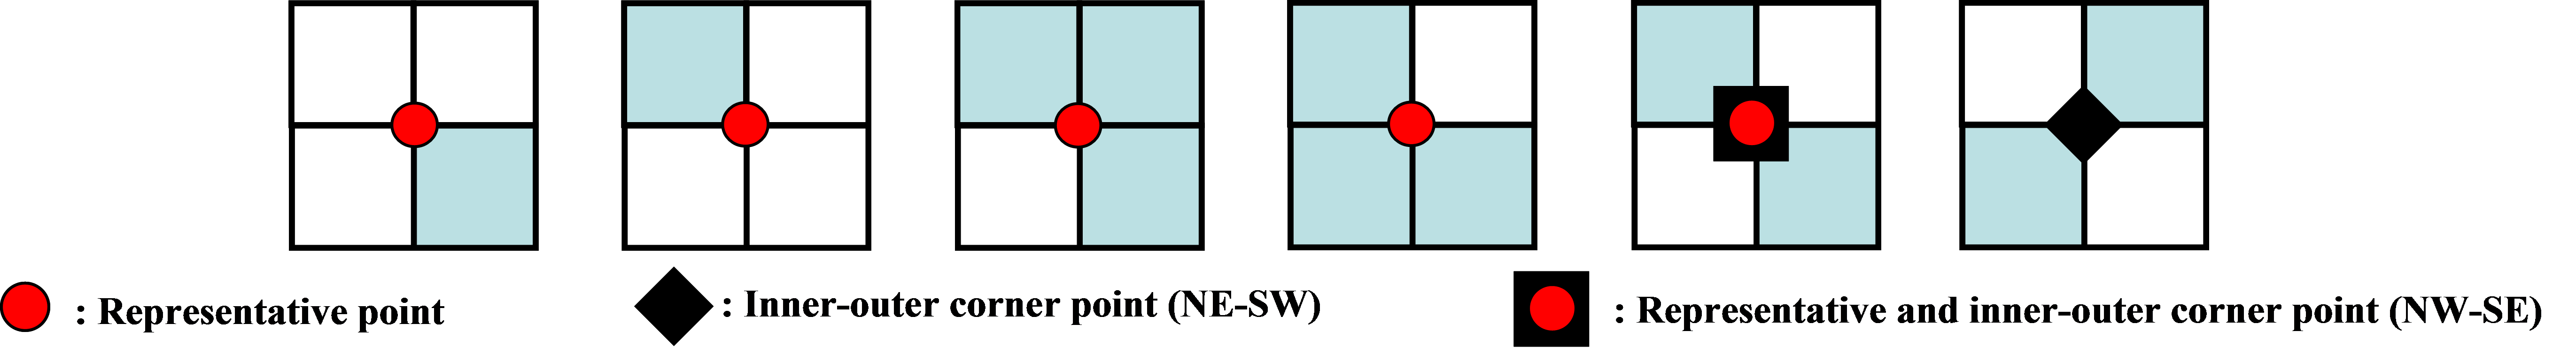
\includegraphics[width=0.24\textwidth]{4.Proposed/fig12-a.png} \label{fig:img12-a} }
	\subfloat[]{ 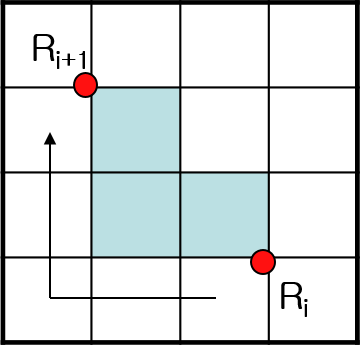
\includegraphics[width=0.24\textwidth]{4.Proposed/fig12-b.png} \label{fig:img12-b} }
	\subfloat[]{ 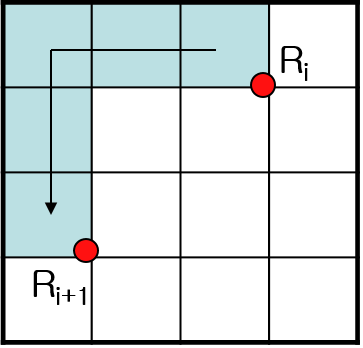
\includegraphics[width=0.24\textwidth]{4.Proposed/fig12-c.png} \label{fig:img12-c} } 
	\subfloat[]{ 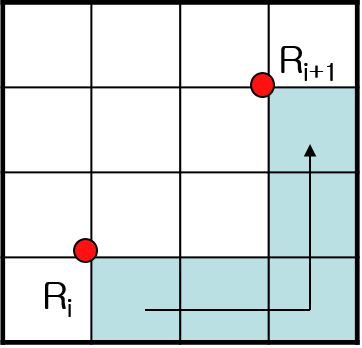
\includegraphics[width=0.24\textwidth]{4.Proposed/fig12-d.png} \label{fig:img12-d} }
	\caption{Contour Pixel Reconstruction. \protect\subref{fig:img12-a} SE \protect\subref{fig:img12-b} NW \protect\subref{fig:img12-c} SW \protect\subref{fig:img12-d} NE}
	\label{fig:image12}
\end{figure}

% The methods in figure \JHMEMO{13} are the basic methods for restoring the contour, but they have a problem in reconstructing the inner corner pixel using three or more representative points. Table \ref{table:ex_innerCornerMissing} and figure \JHMEMO{14} show cases of missing inner corner pixels using sequential representative points $R_i$, $R_{i+1}$, and $R_{i+2}$.

The methods in Figure \ref{fig:image12} are the basic methods employed to restore the contour, but they are problematic when used to reconstruct the inner-corner pixel using three or more representative points. Table \ref{table:ex_innerCornerMissing} and Figure \ref{fig:image13} show cases of the missing inner-corner pixels using sequential representative points $R_i$, $R_{i+1}$, and $R_{i+2}$.

%%% Image 13
\begin{figure}[htbp]
	\centering
	\subfloat[]{ 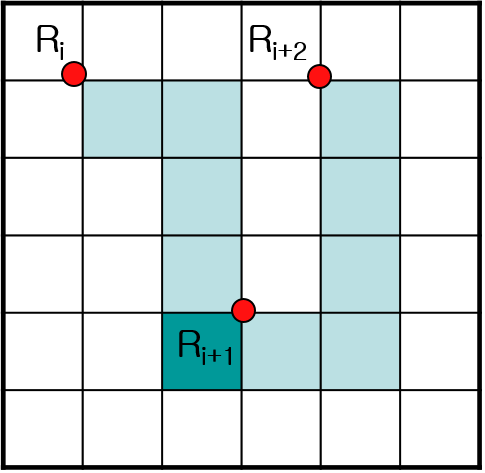
\includegraphics[width=0.24\textwidth]{4.Proposed/fig13-a.png} \label{fig:img13-a} }
	\subfloat[]{ 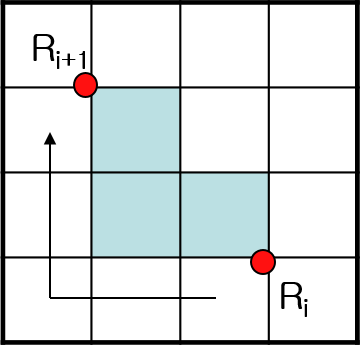
\includegraphics[width=0.24\textwidth]{4.Proposed/fig13-b.png} \label{fig:img13-b} }
	\subfloat[]{ 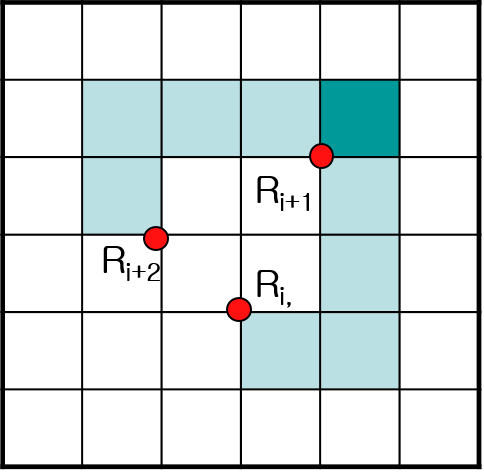
\includegraphics[width=0.24\textwidth]{4.Proposed/fig13-c.png} \label{fig:img13-c} } 
	\subfloat[]{ 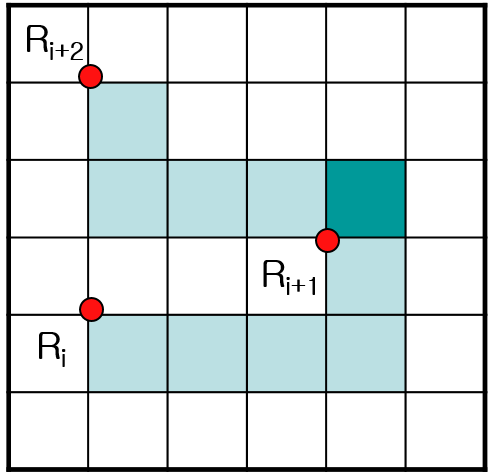
\includegraphics[width=0.24\textwidth]{4.Proposed/fig13-d.png} \label{fig:img13-d} } //
	\subfloat[]{ 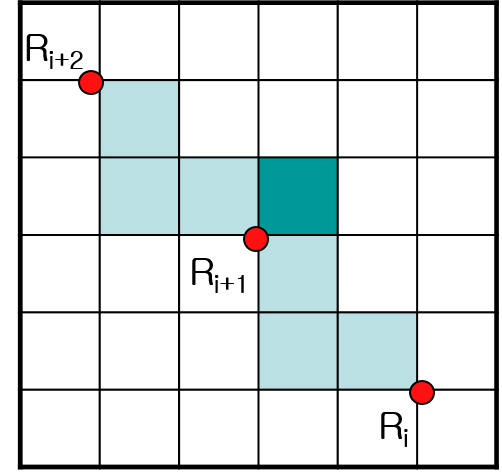
\includegraphics[width=0.24\textwidth]{4.Proposed/fig13-e.png} \label{fig:img13-e} }
	\subfloat[]{ 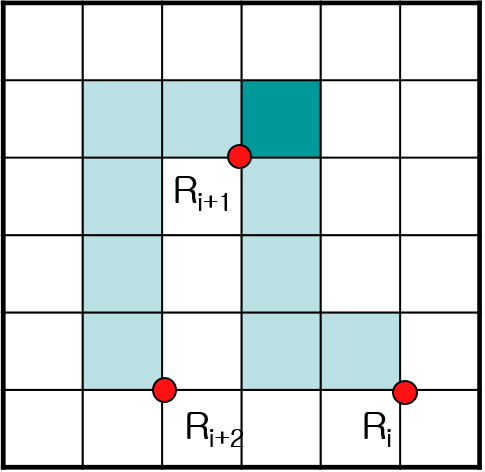
\includegraphics[width=0.24\textwidth]{4.Proposed/fig13-f.png} \label{fig:img13-f} }
	\subfloat[]{ 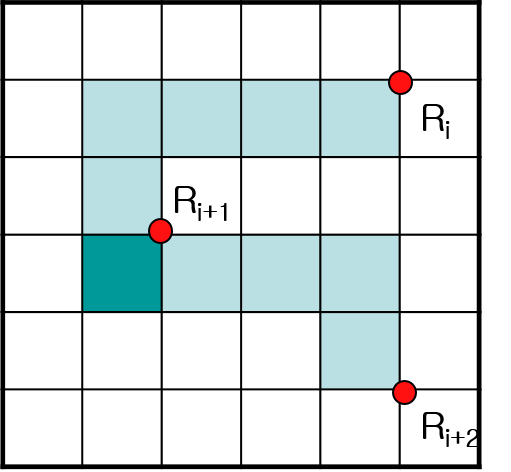
\includegraphics[width=0.24\textwidth]{4.Proposed/fig13-g.png} \label{fig:img13-g} }
	\subfloat[]{ 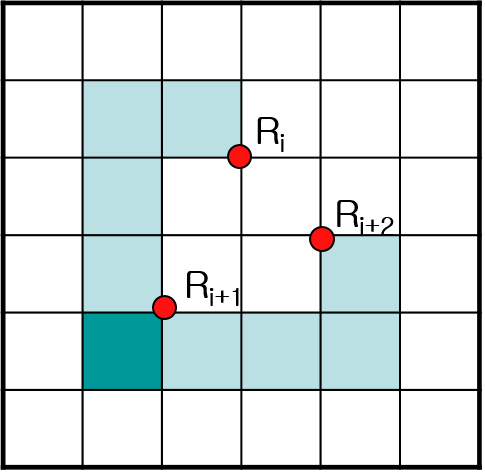
\includegraphics[width=0.24\textwidth]{4.Proposed/fig13-h.png} \label{fig:img13-h} }
	 
	\caption{Restoration Cases for Different Sequences of Representation Points. \protect\subref{fig:img13-a} - \protect\subref{fig:img13-h} Case 1 - 8}
	\label{fig:image13}
\end{figure}

 \begin{table}[h]
	\centering
	\begin{tabularx}{0.7\textwidth}{Y|Y|Y}
		\hline
		Case & $(R_i, R_{i+1})$ & $(R_{i+1}, R_{i+2})$\\
		\hline
		1 & SE & NE \\
		2 & SE & SE \\
		3 & NE & SW \\
		4 & NE & NW \\
		5 & NW & NW \\
		6 & NW & SW \\
		7 & SW & SE \\
		8 & SW & NE \\
		\hline
	\end{tabularx}
	\caption{Examples of Inner Corner Missing}
	\label{table:ex_innerCornerMissing}
\end{table}

% As shown in the figure, the three representative points cannot restore the inner corner pixel $P_m$. Therefore, if the three sequential points form one of the cases in table \ref{table:ex_innerCornerMissing}, $P_m$ of the middle representative point $R_{i+1}$ must be filled with black. 

As shown in the figure, the three representative points cannot restore the inner-corner pixel $P_m$. Therefore, if the three sequential points form one of the cases in Table \ref{table:ex_innerCornerMissing}, $P_m$ of the middle representative point $R_{i+1}$ must be filled with black. 

% This reconstruction method is different from the restoration in the RD code method since the proposed method does not need the RD code but requires only representative points, and their saved sequence naturally replaces the RD code. Therefore, it requires a smaller memory size as compared to the RD code method.

This reconstruction method is different from the restoration approach in the RD code method because the proposed method does not need the RD code, but requires only representative points, and their saved sequence naturally replaces the RD code. Therefore, it requires a smaller memory size when compared to the RD code method.

% \subsubsubsection{Inner-outer corner restoration}
\subsubsection{Inner-outer Corner Restoration}

\JHMEMO{Change the above title to subsubsubsection}


% The restored contour using only the representative points has no inner-outer corners since the inner-outer corner is not considered. For this reason, if there are inner-outer corner points in the data table, as shown in Table \ref{table:data_structure}, the inner-outer corners are generated by using the data $C_j$ with their point coordinates and types. If a pixel restored using the representative points is $o(x, y)$ and $O$ is restored contour, the function of the inner-outer corner restoration, $R_{IO}$, can be obtained as:

The restored contour obtained using only the representative points has no inner-outer corners because the inner-outer corner is not considered. For this reason, if there are inner-outer corner points in the data table, as shown in Table \ref{table:ex_innerCornerMissing}, the inner-outer corners are generated using the data $C_j$ with their point coordinates and types. If a pixel restored using the representative points is $o(x, y)$, and $O$ is the restored contour, the function of the inner-outer corner restoration, $R_{IO}$, can be obtained as

\begin{equation}
R_{IO} = \begin{cases}
O - o(c_{j,x} - 0.5, c_{j,y} - 0.5) - o(c_{j,x} + 0.5, c_{j,y} + 0.5), \text{where\:} c_{j,T} = ``NW-SE'' \\
O - o(c_{j,x} - 0.5, c_{j,y} + 0.5) - o(c_{j,x} + 0.5, c_{j,y} - 0.5), \text{where\:} c_{j,T} = ``NE-SW'' \\
\end{cases}
\label{eq:r_io}
\end{equation}

%!TEX root = ../Fast_Contour_Tracing_Algorithm.tex
% -*- root: ../Fast_Contour_Tracing_Algorithm.tex -*-

\section{Experimental Result}

% For comparing the proposed algorithm with conventional algorithms, we perform experiment for determining their accuracy, speed, and stored data size. Table \ref{table:exp_environment} shows the experimental environment.

To compare the proposed algorithm with conventional algorithms, we perform an experiment to determine their accuracy, speed, and stored data size. Table \ref{table:exp_environment} shows the experimental environment.

\begin{table}[h]
	\centering
	\begin{tabularx}{0.9\textwidth}{L{4cm}L{20cm}}
		\toprule
		  &  Desktop \\ 
		\midrule
		CPU & Intel(R) Core(TM) i7-2600K CPU @ 3.40GHz  \\
		Memory & 14.0 GB \\  
		HDD & Seagate 1TB Momentus ST1000LM024 \\
		O/S & Microsoft Windows 7 \\
		Development & Microsoft Visual Studio 2013 \\ 
		\bottomrule
	\end{tabularx}
	\caption{Experimental Environment}
	\label{table:exp_environment}
\end{table}	

% We experimented on nine CCITT standard fax images with 200 DPI (dots per inch) \textcolor{red}{[14]}. All these images have $1,728 \times 2,339$ pixels and a file size of 11,842 KB. Table \ref{table:ccitt} shows the document type of these images and the total number of contour pixels. We used these large sized images because they a number of various types of contours, and they are useful to compare the efficiencies with regard to parameters such as processing time and accuracy of the trace results of the contour tracing algorithms.

We experimented on nine CCITT standard fax images with 200 dots per inch (dpi) \textcolor{red}{[14]}. All of these images have $1,728 \times 2,339$ pixels and a file size of $11,842 KB$. Table \ref{table:ccitt} shows the document type of these images and the total number of contour pixels. We used these large-sized images because they have various types of contours, which is useful when comparing the efficiencies with regard to parameters such as processing time and the accuracy of the trace results of the contour-tracing algorithms.

\begin{table}[h]
	\centering
	\begin{tabularx}{1.0\textwidth}{C{3cm}YY}
		\toprule
		Index & Type & Total number of contour pixels \\
		\midrule
		1 & Business letter & 81,189 \\
		2 & Circuit diagram & 50,825 \\
		3 & Sales order table & 152,489 \\
		4 & French document & 312,812 \\
		5 & Technical paper & 157,377 \\
		6 & Technical graph & 98,579 \\
		7 & Japanese document & 283,717 \\
		8 & Handwritten memo & 97,031 \\
		9 & Facsimile test chart & 453,721 \\
		\bottomrule
	\end{tabularx}
	\caption{CCITT Fax Standard Images}
	\label{table:ccitt}
\end{table}	

% In order to compare the proposed algorithm with conventional algorithms, we used the experimental method described in \cite{Danielsson1981Improvement} for determining the start pixels of the outer and inner contours of the images. In other words, whenever any untraced contour pixel is searched using a raster scan from the left-top to the right-bottom of the images, this pixel is regarded as the start pixel and the tracer starts contour tracing. If the contour is an outer contour, the tracer's initial direction is assigned as East (``E''). On the contrary, in the case of the inner contour of an object e.g., ``e,'' ``p,'' ``q,'' ``R,'' and ``o,'' the tracer's initial direction is assigned as West (``W''), as shown in figure \textcolor{red}{2 (a)}.

In order to compare the proposed algorithm with conventional algorithms, we used the experimental method described in Ref. \cite{Danielsson1981Improvement} to determine the start pixels of the outer and inner contours of the images. In other words, whenever any untraced contour pixel is searched using a raster scan from the left top to the right bottom of the images, this pixel is regarded as the start pixel, and the tracer starts contour tracing. If the contour is an outer contour, the tracer's initial direction is assigned as East (``E''). On the contrary, in the case of the inner contour of an object, e.g., ``e,'' ``p,'' ``q,'' ``R,'' and ``o,'' the tracer's initial direction is assigned as West (``W''). 

% In the experiments, we did not consider the TPA, since the initial condition of the TPA\cite{Ghuneim2015Contour,Pavlidis2012Algorithms} is that it must start with white left (``L''), left-rear (``W''), and right-rear (``R'') pixels, which is not satisfied in some of the inner contours. Figure \ref{fig:image14} shows an example of this violation. In our experimental situation, there were many cases in which such conditions were not satisfied; therefore, we could not perform identical experiments and meaningful data was not obtained for comparing the trace results with those of the other methods. 

In the experiments, we did not consider the TPA because the initial condition of the TPA [7,9] is that it must start with white left (``L''), left-rear (``W''), and right-rear (``R'') pixels, which is not satisfied in some of the inner contours. Figure \ref{fig:image14} shows an example of this violation. In our experiments, there were many cases for which these conditions were not satisfied. Therefore, we could not perform identical experiments, and meaningful data were not obtained for comparing the trace results with those of the other methods. 

\begin{figure}[htbp]
	\centering
	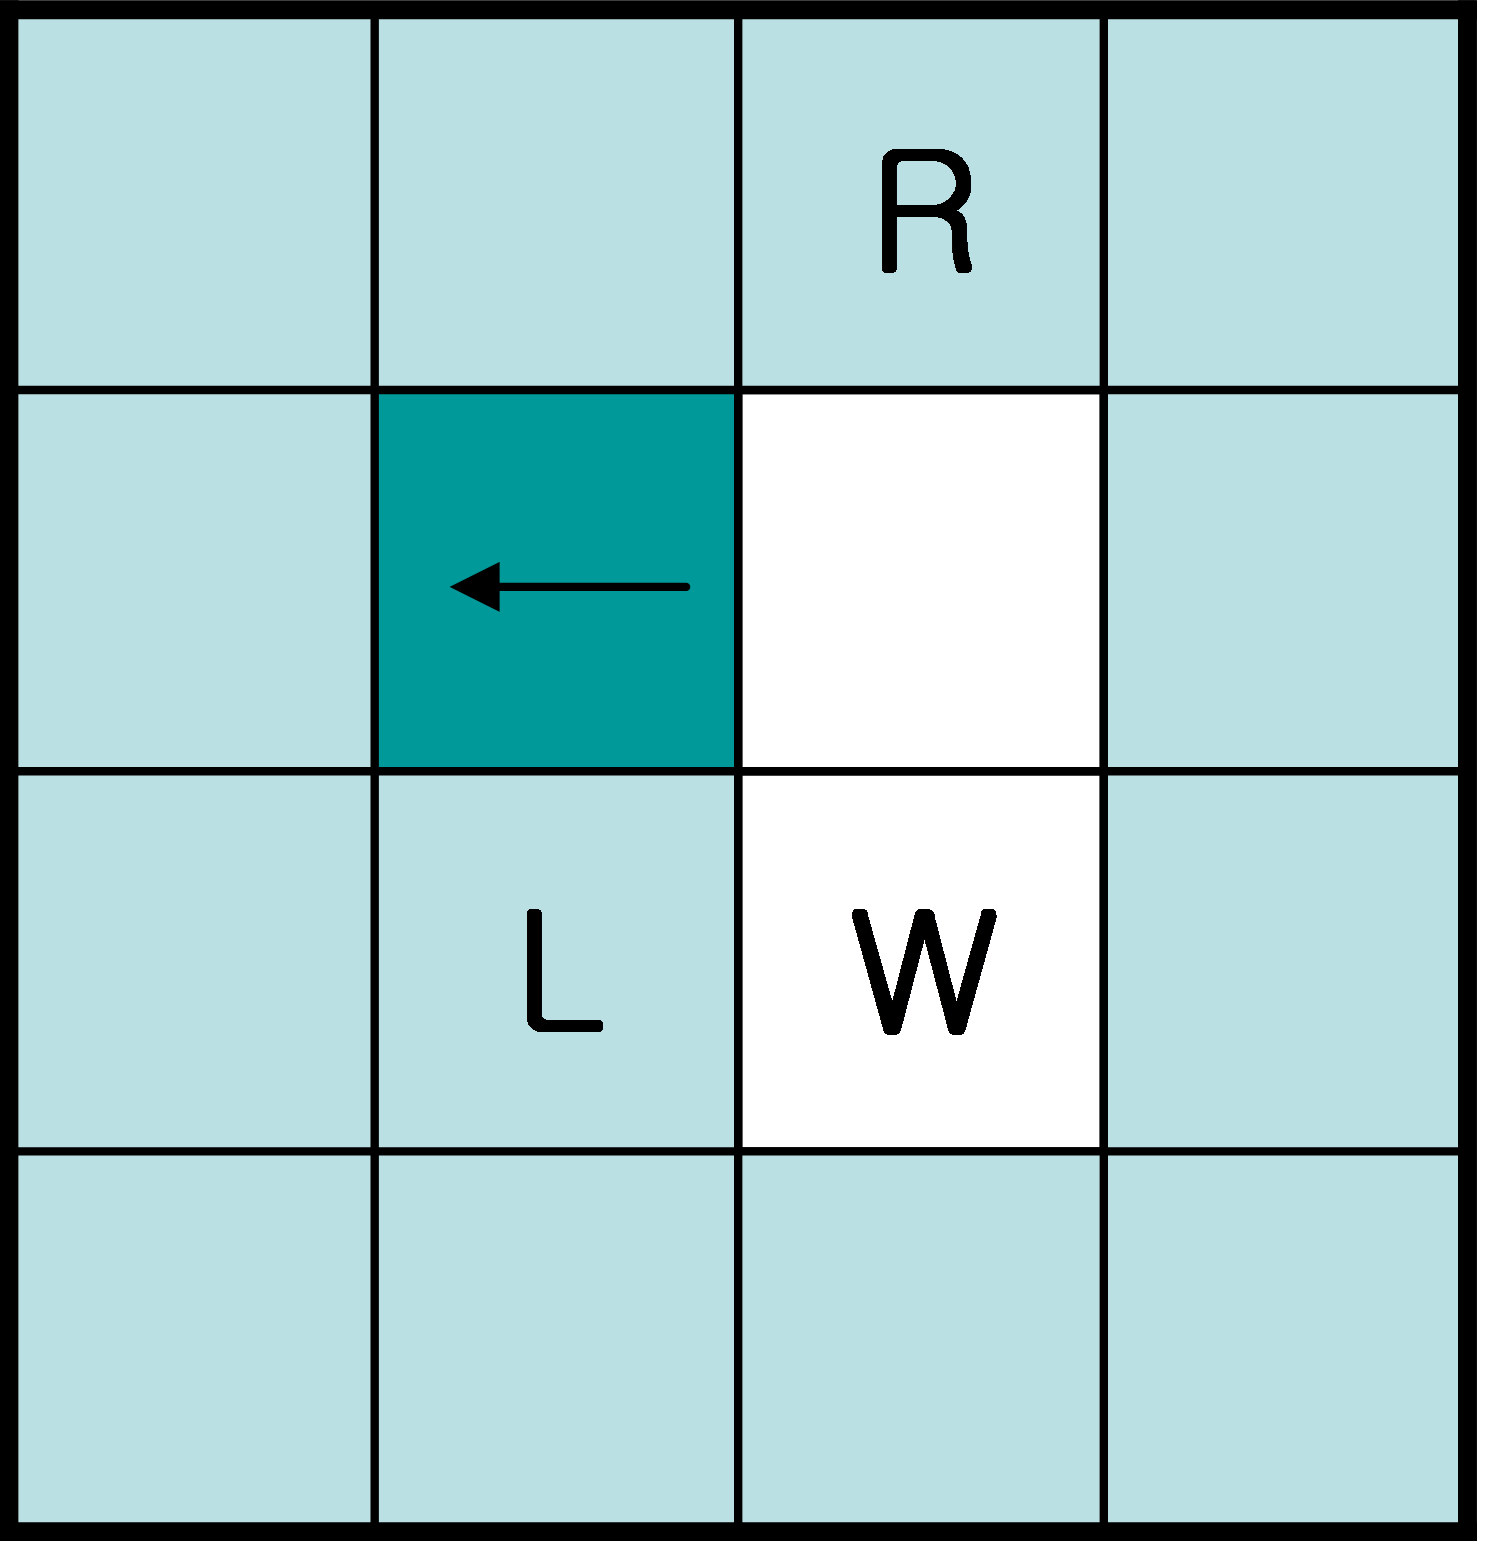
\includegraphics[width=0.3\textwidth]{5.ExperimentalResult/fig14.png}
	\caption{Problem with TPA.}
	\label{fig:image14}
\end{figure}

\subsection{Accuracy}

% The accuracy of contour tracing involves determining how accurately the tracing algorithm traces, and we measure it by counting the number of pixels traced. Firstly, we apply each algorithm to the test images and mark the tracing on the images. Then we count all the marked contour pixels in the images. Therefore, even if a pixel is traced several times, it is counted only once. Table \JHMEMO{7} shows the results of the comparison between the proposed algorithm and the conventional ones. In the table, \JHMEMO{``total number''} implies the total number of contour pixels, including the inner corner, outer corner, inner-outer corner, and straight line pixels. In this result, the MNT and RSA traced the least number of pixels as contours because they could not trace the inner corner pixels. the SBF has inconsistencies with regard to the inner-outer corner and inner corner types; therefore, it traced lesser number of pixels as compared to the ISBF and proposed algorithm.  Further, the MSBF has inner corner inconsistencies that are similar to those of the SBF; the MSBF traced lesser number of pixels as compared to the proposed algorithm and ISBF. The proposed algorithm shows that $99.5\%$ of the total contour pixels were found to be the same as those in the case of the ISBF and it has the maximum total number of traced contour pixels. In conclusion, the proposed algorithm produced the best results with regard to tracing accuracy.

The accuracy of contour tracing involves determining how accurately the tracing algorithm traces, and we measure it by counting the number of pixels traced. First, we apply each algorithm to the test images and mark the tracing on the images. Then, we count all the marked contour pixels in the images. Therefore, even if a pixel is traced several times, it is counted only once. Table Table \JHMEMO{7} shows the results of the comparison between the proposed algorithm and the conventional ones. In the table, ``Total number'' implies the total number of contour pixels, including the inner corner, outer corner, inner-outer corner, and straight-line pixels. In this result, the MNT and RSA traced the least number of pixels as contours because they could not trace the inner-corner pixels. The SBF has inconsistencies with regard to the inner-outer corner and inner-corner types. Therefore, it traced fewer pixels when compared to the ISBF and proposed algorithm. Further, the MSBF has inner-corner inconsistencies that are similar to those of the SBF, and the MSBF traced fewer pixels when compared to the proposed algorithm and ISBF. The proposed algorithm shows that $99.5\%$ of the total contour pixels were found to be the same as those in the case of the ISBF, and it has the maximum total number of traced contour pixels. In conclusion, the proposed algorithm produced the best results with regard to tracing accuracy.

%%% Figure 15
\begin{figure}[htbp]
	\centering
	\subfloat[]{ 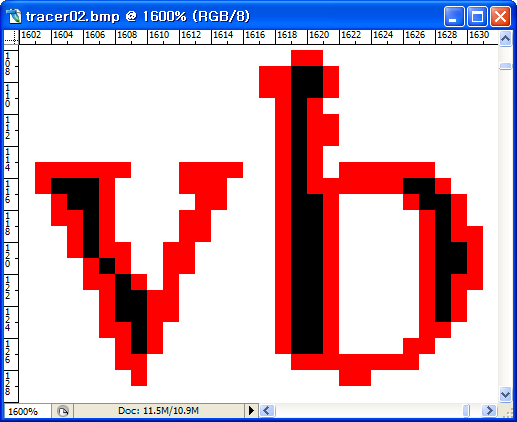
\includegraphics[width=0.3\textwidth]{5.ExperimentalResult/fig15-a.png} \label{fig:img15-a} }
	\subfloat[]{ 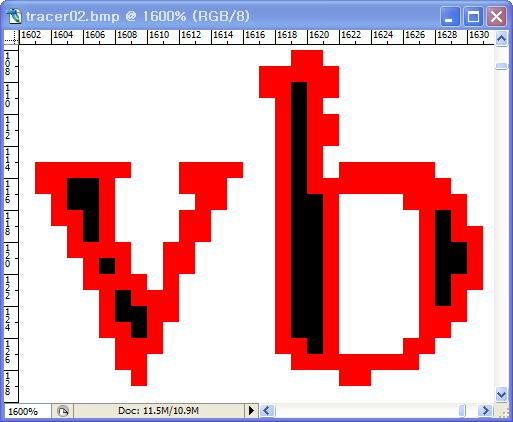
\includegraphics[width=0.3\textwidth]{5.ExperimentalResult/fig15-b.png} \label{fig:img15-b} }

	\caption{Comparison with Contour Tracing. \protect\subref{fig:img15-a} MSBF \protect\subref{fig:img15-b} Proposed method}
	\label{fig:image15}
\end{figure}

% Figure 16 shows the traced images resulting from the MSBF and proposed algorithm. In this figure, (a) could not trace some of the inner corner pixels but (b) traced all the corner pixel types without any inconsistency. Moreover, as the proposed algorithm can classify each corner type, it can trace the selected type of contour pixels by omitting some cases, as shown in figure 9 (b). For example, if we remove the tracing cases (1) and (6) from the other cases, we can obtain a result without inner corner tracing, and it is the same as the result of the MNT and RSA. Figure \textcolor{red}{17 (b)} shows an image that is traced using the proposed algorithm without inner corners, and it shows that the image is consistently traced without inner corners.

Figure \ref{fig:image15} shows the traced images resulting from the MSBF and proposed algorithm. In this figure, in \ref{fig:img15-a}, it was not possible to trace some of the inner corner pixels, but in \ref{fig:img15-b}, it was possible to trace all the corner-pixel types without any inconsistency. Moreover, as the proposed algorithm can classify each corner type, it can trace the selected type of contour pixels by omitting some cases, as shown in Figure \ref{fig:img9-b}. For example, if we remove the tracing cases (1) and (6) from the other cases, we can obtain a result without inner-corner tracing, and it is the same as the result of the MNT and RSA. Figure \ref{fig:img16-b} shows an image that was traced using the proposed algorithm without inner corners, and it shows that the image is consistently traced without inner corners.

%%% Figure 16
\begin{figure}[htbp]
	\centering
	\subfloat[]{ 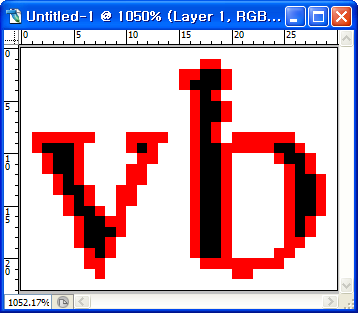
\includegraphics[width=0.3\textwidth]{5.ExperimentalResult/fig16-a.png} \label{fig:img16-a} }
	\subfloat[]{ 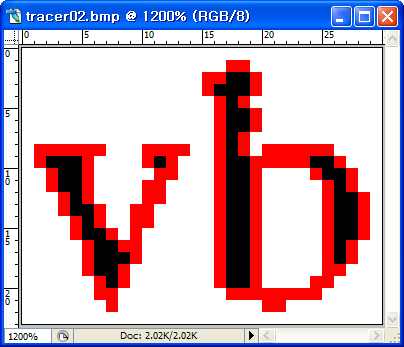
\includegraphics[width=0.3\textwidth]{5.ExperimentalResult/fig16-b.png} \label{fig:img16-b} }

	\caption{Comparison with Contour Tracing. \protect\subref{fig:img16-a} MNT \protect\subref{fig:img16-b} Proposed method (without inner corners)}
	\label{fig:image16}
\end{figure}


%%%%%%%%%%%%%%%%%%%%%%%%%%%%%%%%%%%%%%%%%%%%%%%%%%%%%%%%%%%%%%%%%%%%%%%%%%%
\subsection{Speed}

% In order to measure the tracing time for each algorithm, we performed each algorithm 10 times per image and calculated the average time. We used the GetTickCount() function supported by Microsoft Visual C++ 6.0 to measure the processing time. Tables \textcolor{red}{8 and 9} show the average processing time of each algorithm used for tracing the images, and a linear model for estimating the process time as the number of traced pixels increases by using the least-square estimation (LSE) method. In the tables, the average processing time per traced contour pixel is obtained by dividing the total processing time by the total number of traced contour pixels. They are measured on the desktop and notebook separately.

In order to measure the tracing time for each algorithm, we performed each algorithm 10 times per image and calculated the average time. We used the \JHMEMO{$GetTickCount()$} function supported by \JHMEMO{Microsoft Visual C++ 6.0} to measure the processing time. Tables \JHMEMO{8 and 9} show the average processing time of each algorithm used for tracing the images, and a linear model for estimating the process time as the number of traced pixels increases using the least-square estimation (LSE) method. In the tables, we obtain the average processing time per traced contour pixel by dividing the total processing time by the total number of traced contour pixels.

% Moreover, figure \textcolor{red}{18} illustrates a graph that uses data from tables \textcolor{red}{7 to 9}. As shown in figures \textcolor{red}{18 (a) and (b)}, the proposed algorithm had the best performance in the case of the desktop, i.e., it had the least average processing time and showed the least increase in the ratio of process time to number of traced contour pixels, as shown in the LSE. In particular, although the proposed algorithm traced most of the numerous contour pixels in each image, it has the best or good performance when compared with the conventional algorithms. On the contrary, the SBF had the least average processing time for images and the least ratio from the LSE in the case of the notebook, and the proposed algorithm is second in rank based on the average processing time and LSE. from these experimental results the SBF is not the best algorithm for the note book because the ratio of the number of traced contour pixels is only approximately $92\%$ of the proposed algorithm. Due to this reason, the proposed algorithm has better performance than the other algorithms for the number of traced contour pixels and the processing time.

\JHMEMO{
Figure \JHMEMO{18} illustrates a graph that uses data from Tables \JHMEMO{7-9}. As shown in Figures \JHMEMO{18(a) and (b)}, the proposed algorithm has the best performance in the case of the desktop PC, i.e., it had the least average processing time and showed the smallest increase in the ratio of the process time to the number of traced contour pixels, as shown in the LSE. In particular, although the proposed algorithm traced most of the contour pixels in each image, it has the best or a good performance when compared to the conventional algorithms. On the contrary, for the notebook PC, the SBF had the smallest average processing time for images and the smallest ratio from the LSE. In addition, the proposed algorithm is ranked second based on the average processing time and LSE. From these experimental results, the SBF algorithm is not ideal for the notebook PC because the ratio of the number of traced contour pixels is only approximately $92\%$ of the value of the proposed algorithm. Therefore, the proposed algorithm has a better performance than the other algorithms for the number of traced contour pixels and the processing time. 
}

%%%%%%%%%%%%%%%%%%%%%%%%%%%%%%%%%%%%%%%%%%%%%%%%%%%%%%%%%%%%%%%%%%%%%%%%%%%
\subsection{Reduced Memory}

% The proposed algorithm does not save all the contour pixels, but it saves only the representative points and the inner-outer corner pixels. Table \textcolor{red}{10} shows the data size acquired from the above experiments on CCITT standard fax images. It shows the data sizes of traced contour pixels and its compressed data. The number of traced contour pixels $(A)$, which are same results from table \textcolor{red}{7} and the $C$ and $D$ in the table are numbers of the representative points and the inner-outer corner points of the traced contour pixels. $A$ and $C$ are the number of $(x, y)$ coordinates, and $D$ represents the number of inner-outer corners that comprise $(x, y)$ coordinates and the type of inner-outer corner. The benefit of storing only the representative points based on the vertex of the contour pixel is that it can dramatically reduce the data size. This experimental results showed that the proposed algorithm reduced the data size to {19~60\%} of the memory used when all the contour pixels were stored, as shown in Table \textcolor{red}{10}.

The proposed algorithm does not save all of the contour pixels, but it saves only the representative points and the inner-outer corner pixels. Table \ref{table:table10} shows the data size acquired from the above experiments performed using CCITT standard fax images. It shows the data sizes of traced contour pixels and their compressed data. The number of traced contour pixels (A), which are the same results from \JHMEMO{Table 7}, and $C$ and $D$ in the table indicate the number of representative points and inner-outer corner points of the traced contour pixels. $A$ and $C$ are the number of $(x, y)$ coordinates, and $D$ represents the number of inner-outer corners that comprise $(x, y)$ coordinates and the type of inner-outer corner. The benefit of storing only the representative points based on the vertex of the contour pixel is that it can significantly reduce the data size. The experimental results obtained show that the proposed algorithm reduced the data size to $19-60\%$ of the memory used when all of the contour pixels were stored, as shown in Table \ref{table:table10}.

%%% Table 10
%!TEX root = ../Fast_Contour_Tracing_Algorithm.tex
% -*- root: ../Fast_Contour_Tracing_Algorithm.tex -*-

% \begin{table}[]
% \scriptsize
% \centering
% \caption{Comparison Between Total Contour Pixels and Representative Points.}
% \label{table:table10}
% \begin{tabularx}{1.0\textwidth}{rR{2.1cm}R{2.0cm}R{2.9cm}R{3.0cm}R{2.5cm}R{2cm}}

% \toprule
% \multirow{2}{*}{} & \multicolumn{2}{l}{Entire contour pixels} & \multicolumn{3}{l}{Compressed data} & \multirow{2}{*}{Ratio ($\%$) ($E / B \times 100$) }	\\
% 				  & \multicolumn{1}{l}{Number of contour pixels ($A$)} & Data size ($B = A \times 2$) & Number of representative points ($C$) & Number of Inner outer corner points ($D$) & Data size ($E = C \times 2 + D \times 3$) & \\
% \midrule
% \#1               & 81,188                         & 162,376                      & 21,206                                & 61                                        & 42,595  & 26.23 \\
% \#2               & 50,824                         & 101,648                      & 12,695                                & 21                                        & 25,453  & 25.04 \\
% \#3               & 152,487                        & 304,974                      & 30,181                                & 53                                        & 60,521  & 19.84 \\
% \#4               & 312,812                        & 625,624                      & 86,953                                & 442    & 175,232 & 28.01 \\
% \#5               & 157,374                        & 314,748                      & 37,386                                & 113    & 75,111  & 23.86 \\
% \#6               & 98,566                         & 197,132                      & 18,464                                & 104    & 37,240  & 18.89 \\
% \#7               & 283,551                        & 567,102                      & 84,484                                & 1,539  & 173,585 & 30.61 \\
% \#8               & 97,015                         & 194,030                      & 21,928                                & 104    & 44,168  & 22.76 \\
% \#10              & 445,975                        & 891,950                      & 158,529                               & 75,425 & 543,333 & 60.92 \\
% \bottomrule

% \end{tabularx}
% \end{table}


% Please add the following required packages to your document preamble:
% \usepackage{multirow}
% \usepackage{graphicx}
\begin{table}[]
\centering
\caption{Comparison Between Total Contour Pixels and Representative Points.}
\label{table:table10}
\resizebox{\textwidth}{!}{%
\begin{tabular}{rrrrrrr}

\toprule

\multicolumn{1}{l}{} & \multicolumn{2}{l}{Entire contour pixels}                                                             & \multicolumn{3}{l}{Compressed data}                                   & \multicolumn{1}{l}{\multirow{2}{*}{\bigcell{Ratio ($\%$)\\($E / B \times 100$)}}} \\

\multicolumn{1}{l}{} & \bigcell{Number of\\contour pixels ($A$)} & \bigcell{Data size\\($B = A \times 2$)} & \bigcell{Number of\\representativepoints ($C$)} & \bigcell{Number of Inner outer\\corner points ($D$)} & \bigcell{Data size\\($E = C \times 2 + D \times 3$)} & \multicolumn{1}{l}{}                            \\


\midrule
\#1                  & 81,188                                             & 162,376                                          & 21,206                & 61                    & 42,595                & 26.23                                           \\
\#2                  & 50,824                                             & 101,648                                          & 12,695                & 21                    & 25,453                & 25.04                                           \\
\#3                  & 152,487                                            & 304,974                                          & 30,181                & 53                    & 60,521                & 19.84                                           \\
\#4                  & 312,812                                            & 625,624                                          & 86,953                & 442                   & 175,232               & 28.01                                           \\
\#5                  & 157,374                                            & 314,748                                          & 37,386                & 113                   & 75,111                & 23.86                                           \\
\#6                  & 98,566                                             & 197,132                                          & 18,464                & 104                   & 37,240                & 18.89                                           \\
\#7                  & 283,551                                            & 567,102                                          & 84,484                & 1,539                 & 173,585               & 30.61                                           \\
\#8                  & 97,015                                             & 194,030                                          & 21,928                & 104                   & 44,168                & 22.76                                           \\
\#10                 & 445,975                                            & 891,950                                          & 158,529               & 75,425                & 543,333               & 60.92                                          \\
\bottomrule
\end{tabular}
}
\end{table}

%%%%%%%%%%%%%%%%%%%%%%%%%%%%%%%%%%%%%%%%%%%%%%%%%%%%%%%%%%%%%%%%%%%%%%%%%%%
\subsection{Restoration}

% Figure \ref{fig:image19} shows an example of retrieval points and a restoration result obtained by using the proposed restoration algorithm. Figure \ref{fig:img19-a} is an example image that has all the contour pixel types, and it depicts the representative points and inner-outer corner points for contour description and restoration. This image has two contours, namely, an outer contour and an inner contour that includes two inner-outer corners. Table \textcolor{red}{11} describes these data and figure \textcolor{red}{18 (b)} shows the restoration results, which are retrieved using the data from table \textcolor{red}{11}. In the figure, the restored contour accurately represents the original contour pixels.

Figure \ref{fig:image19} shows an example of the retrieval points and a restoration result obtained using the proposed restoration algorithm. Figure \ref{fig:img19-a} is an example image that has all of the contour pixel types, and it depicts the representative points and inner-outer corner points for contour description and restoration. This image has two contours, namely an outer contour and an inner contour that includes two inner-outer corners. Table \ref{table:table11} describes these data and Figure \ref{fig:img19-b} shows the restoration results, which were retrieved using the data from Table \ref{table:table11}. In the figure, the restored contour accurately represents the original contour pixels.

%%% Image 19
\begin{figure}[htbp]
	\centering
	\subfloat[]{ \includegraphics[width=7cm, height=6cm]{5.ExperimentalResult/fig19_a.png} \label{fig:img19-a} }
	\subfloat[]{ \includegraphics[width=7cm, height=5.25cm]{5.ExperimentalResult/fig19_b.png} \label{fig:img19-b} }
	 
	\caption{Example of Restoration of Contour Pixels. \protect\subref{fig:img19-a} Original image and its saved points for restoration      \protect\subref{fig:img19-b} Restoration by saved data}
	\label{fig:image19}
\end{figure}

%%% Table 11
%!TEX root = ../Fast_Contour_Tracing_Algorithm.tex
% -*- root: ../Fast_Contour_Tracing_Algorithm.tex -*-

% Please add the following required packages to your document preamble:
% \usepackage{multirow}
\begin{table}[]
\centering
\caption{Saved Data}
\label{table:table11}
\resizebox{\textwidth}{!}{%

\begin{tabular}{rrrllllllll}
\toprule
\multirow{3}{*}{i} & \multicolumn{5}{c}{Contour \#1. (outer contour)}                 & \multicolumn{5}{c}{Contour \#2. (inner contour)}                 \\ 
                   & \multicolumn{2}{c}{$R_i$} & \multicolumn{2}{c}{$C_i$} &          & \multicolumn{2}{c}{$R_i$} & \multicolumn{2}{c}{$C_i$} &          \\
                   & $x$           & $y$           & $x$           & $y$           & type     & $x$           & $y$           & $x$           & $y$           & type     \\
\midrule 
1                  & 3.5         & 1.5         & 9.5         & 9.5         & NE-SW    & 5.5         & 9.5         & 5.5         & 9.5         & NW-SE    \\
2                  & 5.5         & 3.5         & 5.5         & 9.5         & NW-SE    & 9.5         & 5.5         & 9.5         & 9.5         & NE-SW    \\
3                  & 9.5         & 1.5         &             &             &          &             &             &             &             &          \\
4                  & 11.5        & 3.5         &             &             &          &             &             &             &             &          \\
5                  & 13.5        & 7.5         &             &             &          &             &             &             &             &          \\
6                  & 11.5        & 9.5         &             &             &          &             &             &             &             &          \\
7                  & 9.5         & 11.5        &             &             &          &             &             &             &             &          \\
8                  & 5.5         & 9.5         &             &             &          &             &             &             &             &          \\
9                  & 3.5         & 7.5         &             &             &          &             &             &             &             &          \\
10                 & 1.5         & 3.5         &             &             &          &             &             &             &             &          \\
\bottomrule
\end{tabular}
}
\end{table}

% Figure \ref{fig:image20} shows the result for the CCITT \#1 image using the proposed restoration algorithm. Figure \ref{fig:img20-a} represents the result of contour tracing and \ref{fig:img20-b} depicts the result of restoration from the compressed contour data. To verify the identity, we compared the contour pixels of the two images and they are identical with regard to the number of contour pixels and the pixel coordinates, i.e., the contour pixels in the restoration result is the same as the original contour pixels. As shown in figures \ref{fig:image20} \textcolor{red}{figures 19 and 20}, these experiments proved that the proposed algorithm could trace the inner and outer contours, and it could store the results using lesser memory by storing only the representative points and inner-outer corner points instead of all the contour pixels; moreover, it could accurately restore all the contour pixels correctly from the compressed data. Besides, as shown in \cite{Miyatake1997Contour}, compressed data based on vertex contours guarantee precise enlarging.

Figure  \ref{fig:image20} shows the result obtained for the CCITT \#1 image using the proposed restoration algorithm. Figure \ref{fig:img20-a} represents the contour-tracing result, and \ref{fig:img20-b} depicts the result of restoration from the compressed contour data. To verify the identity, we compared the contour pixels of the two images, and found that they are identical with regard to the number of contour pixels and the pixel coordinates, i.e., the contour pixels in the restoration result are the same as the original contour pixels. As shown in Figures \ref{fig:image19} and \ref{fig:image20}, these experiments proved that the proposed algorithm could trace the inner and outer contours. Further, it was able to store the results using less memory by storing only the representative points and inner-outer corner points instead of all the contour pixels; moreover, it could correctly restore all the contour pixels from the compressed data. Besides, as shown in [11], compressed data based on vertex contours guarantee precise enlarging.

%%% Image 20
\begin{figure}[htbp]
	\centering
	\subfloat[]{ \includegraphics[width=0.5\textwidth]{5.ExperimentalResult/fig20_a.png} \label{fig:img20-a} }
	\subfloat[]{ \includegraphics[width=0.5\textwidth]{5.ExperimentalResult/fig20_b.png} \label{fig:img20-b} }
	 
	\caption{Result of Experiment for CCITT \#1. Red Pixels are Contour Pixels. \protect\subref{fig:img20-a} Result of contour tracing \protect\subref{fig:img20-b} Result of contour restoration}
	\label{fig:image20}
\end{figure}



%%%%%%%%%%%%%%%%%%%%%%%%%%%%%%%%%%%%%%%%%%%%%%%%%%%%%%%%%%%%%%%%%
\subsection{Limitations}

%%% Image 21
\begin{figure}[htbp]
	\centering
	\subfloat[]{ \includegraphics[width=4.5cm, height=4.5cm]{5.ExperimentalResult/fig21-a.png} \label{fig:img21-a} }
	\subfloat[]{ \includegraphics[width=4.5cm, height=4.5cm]{5.ExperimentalResult/fig21-b.png} \label{fig:img21-b} }
	\subfloat[]{ \includegraphics[width=4.5cm, height=4.5cm]{5.ExperimentalResult/fig21-c.png} \label{fig:img21-c} }
	 
	\caption{Example of Untraed Contour Pixels Caused by Missing Starting Pixel CCITT Image \#9 From $(1093, 1766)$ to $(1108, 1780)$. \protect\subref{fig:img21-a} Original image \protect\subref{fig:img21-b} Traced by ISBF \protect\subref{fig:img21-c} Traced by the proposed algorithm}
	\label{fig:image21}
\end{figure}

%%% Image 22
\begin{figure}[htbp]
	\centering
	\includegraphics[width=0.6\textwidth]{5.ExperimentalResult/fig22.png}
	\caption{Result of Proposed Algorithm by using Bidirectional Scanning.}
	\label{fig:image22}
\end{figure}

\JHMEMO{See comment!}
%\JHMEMO{21 b와 c 가 차이가 없어 보임, 22에서 지적한 점이 c에서 찾아져야 할 것 같음}

% In the experiments, there were some missing contour pixels that did not satisfy the experimental conditions described in \cite{Danielsson1981Improvement}. In figures \ref{fig:img21-b} and \ref{fig:img21-c}, there are eight untraced contour pixels because the horizontal scan line cannot find a starting pixel for the contour under some conditions. In other words, since the scan line seeks an untraced black pixel with an adjacent white pixel on the horizontal line, if the untraced contour pixel which is between two black pixels in the horizontal direction has an adjacent white pixel in the vertical and/or diagonal direction, the untraced contour pixel cannot be considered as the starting pixel. Therefore, as shown in \textcolor{red}{Table 7}, the missing contour pixels remain after running the proposed algorithm and the untraced contour pixels of other algorithms are also included in the missing contour pixels due to the same problem. In particular, image \#9 has the largest number of missing contour pixels because it has many one-pixel-sized chessboard patterns that comprise inner-outer corner pixels. The chessboard pattern consists of one-pixel-sized inner-outer corner pixels, which tend to cause the missing start pixel problem. 

In the experiments, there were missing contour pixels that did not satisfy the experimental conditions described in [12]. In Figures \ref{fig:img21-b} and \ref{fig:img21-c}, there are eight untraced contour pixels because the horizontal scan line cannot find a starting pixel for the contour under certain conditions. In other words, because the scan line seeks an untraced black pixel with an adjacent white pixel on the horizontal line, if the untraced contour pixel that is between two black pixels in the horizontal direction has an adjacent white pixel in the vertical and/or diagonal direction, the untraced contour pixel cannot be considered as the starting pixel. Therefore, as shown in \JHMEMO{Table 7}, the missing contour pixels remain after running the proposed algorithm, and the untraced contour pixels of other algorithms are included in the missing contour pixels for the same reason. In particular, image \#9 has the largest number of missing contour pixels because it has many one-pixel-sized chessboard patterns that comprise inner-outer corner pixels. The chessboard pattern consists of one-pixel-sized inner-outer corner pixels, which tend to cause the missing start-pixel problem. 

% To overcome the problem, we can apply an 8 connection mask to the images for obtaining the starting pixel, but the mask requires many operations. In other words, we made an attempt to measure the performance of multidirection scanning for eliminating the missing contour pixels problem by using vertical and horizontal scans instead of 8 connection mask operation. \textcolor{red}{Table 12} shows the increase in the number of pixels traced by using bidirectional scanning, and \textcolor{red}{Table 13} describes the processing time for this method. Moreover, figure \ref{fig:image22} shows the tracing result obtained by using the proposed algorithm based on bidirectional scanning, and it shows that seven of the missing pixels are traced but still one diagonal connective contour pixel \textcolor{red}{(A)} is untraced. 

To overcome the problem, we applied an eight-connection mask to the images to obtain the starting pixel, but the mask required many operations. In other words, we attempted to measure the performance of multidirection scanning in order to eliminate the missing contour-pixel problem by using vertical and horizontal scans instead of an eight-connection mask operation. Table \ref{table:table12} shows the increase in the number of pixels traced using bidirectional scanning, and \JHMEMO{Table 13} describes the processing time for this method. Moreover, Figure \ref{fig:image22} shows the tracing result that was obtained using the proposed algorithm based on bidirectional scanning, and it shows that seven of the missing pixels are traced, but one diagonal connective-contour pixel (A) remained untraced. 

% In the above tables, bidirectional scanning slightly increases the number of traced contour pixels, but their processing time increases dramatically. Moreover, the proposed algorithm shows acceptable performance in terms of accuracy $(99.5\%)$, although only unidirectional scanning is performed. Hence, unidirectional scanning based on the proposed algorithm is sufficient for application to contour tracing under the condition that a relatively small number of objects are present and real-time tracing such as AR, MR, and recognition-image-based code is performed on small-scale images such as those in a mobile computing environment.

In the above tables, bidirectional scanning slightly increases the number of traced contour pixels, but their processing time increases significantly. Moreover, the proposed algorithm shows acceptable performance in terms of accuracy $(99.5\%)$, although we performed only unidirectional scanning. Hence, unidirectional scanning based on the proposed algorithm is sufficient for application to contour tracing under the condition that relatively few objects are present, and we performed real-time tracing such as AR, MR, and recognition-image-based code on small-scale images such as those in a mobile computing environment.

%!TEX root = ../Fast_Contour_Tracing_Algorithm.tex
% -*- root: ../Fast_Contour_Tracing_Algorithm.tex -*-

% Please add the following required packages to your document preamble:
% \usepackage{booktabs}
% \usepackage{multirow}
\begin{table}[]
\centering
\caption{Increases of Pixels Traced by Bidirectional Scan From One-directional Scan.}
\label{table:table12}

\resizebox{\textwidth}{!}{%

\begin{tabular}{@{}crrlrlrlrlrlrl@{}}
\toprule
      & \multirow{2}{*}{Total Number} & \multicolumn{2}{l}{Proposed} & \multicolumn{2}{l}{ISBF} & \multicolumn{2}{l}{MSBF} & \multicolumn{2}{l}{SBF} & \multicolumn{2}{l}{MNT} & \multicolumn{2}{l}{RSA} \\
      &                               & Number        & \%           & Number      & \%         & Number      & \%         & Number      & \%        & Number      & \%        & Number      & \%        \\ \midrule
\#1   & 81,189                        & 1             & 0.001        & 1           & 0.001      & 1           & 0.001      & 1           & 0.001     & 0           & 0.000     & 0           & 0.000     \\
\#2   & 50,825                        & 0             & 0.000        & 0           & 0.000      & 0           & 0.000      & 0           & 0.000     & 0           & 0.000     & 0           & 0.000     \\
\#3   & 152,489                       & 2             & 0.001        & 2           & 0.001      & 3           & 0.002      & 3           & 0.002     & 1           & 0.001     & 1           & 0.001     \\
\#4   & 312,812                       & 0             & 0.000        & 0           & 0.000      & 0           & 0.000      & 0           & 0.000     & 0           & 0.000     & 0           & 0.000     \\
\#5   & 157,377                       & 3             & 0.002        & 3           & 0.002      & 0           & 0.000      & 0           & 0.000     & 0           & 0.000     & 0           & 0.000     \\
\#6   & 98,579                        & 7             & 0.007        & 7           & 0.007      & 8           & 0.008      & 8           & 0.008     & 1           & 0.001     & 1           & 0.001     \\
\#7   & 283,717                       & 120           & 0.042        & 120         & 0.042      & 67          & 0.024      & 67          & 0.024     & 92          & 0.032     & 92          & 0.032     \\
\#8   & 97,031                        & 12            & 0.012        & 12          & 0.012      & 15          & 0.015      & 15          & 0.015     & 1           & 0.001     & 1           & 0.001     \\
\#9   & 453,721                       & 7,075         & 1.559        & 7,076       & 1.560      & 433         & 0.095      & 444         & 0.098     & 3,414       & 0.752     & 3,414       & 0.752     \\
Total & 1,687,740                     & 7,220         & 0.428        & 7,221       & 0.428      & 527         & 0.031      & 538         & 0.032     & 3,509       & 0.208     & 3,509       & 0.208     \\  
\bottomrule
\end{tabular}
}
\end{table}

%!TEX root = ../Fast_Contour_Tracing_Algorithm.tex
% -*- root: ../Fast_Contour_Tracing_Algorithm.tex -*-

\section{Conclusion}

In this paper, we proposed a contour tracing algorithm to trace contours in low-performance devices such as mobile phones, PDAs, and embedded devices that have a processor with limited computational capability and a small memory capacity. The proposed algorithm traces contour pixels based on the pixel following method, and it can also convert the contour information to compressed data and accurately restore it to the original contour by using the vertex following method. The proposed algorithm repeatedly executes the two tracing stages. first, the tracer moves to the next pixel based on its left and left-rear pixels. Next, it moves based on the front and front-left pixels. With these pixel pairs, the contour pixel can be classified into four types, namely, inner corner, outer corner, inner-outer corner, and straight line, and this classification is used to reduce the computational time for tracing the next contour pixel without duplicated detection of the background pixel. Moreover, based on the classified cases, we can determine the representative points and the inner-outer corner points that are based on the coordinates of the vertices, and we can store the contour data as points in order to reduce the data size. In addition, we proposed a restoration algorithm to retrieve all the contour pixels from the representative points and the inner-outer corner points. It performs accurate restoration and it can also restore the inner-outer corners that were not considered in conventional algorithms such as the RD code method and the PXY method. Another characteristic of the proposed algorithm is that it can trace the desired type of connectivity since it is able to distinguish between the connection types of the contour pixels. For example, the proposed algorithm may trace without inner corners, which is similar to the performance of MNT and RSA.

We experimented with regard to three aspects—accuracy, speed, and saving data. In the results of the experiments, the proposed algorithm had the best performance with regard to the accuracy of contour tracing, i.e., it traced the largest number of contour pixels among the algorithms. Moreover, it showed the least average processing time per contour pixel and good performance with respect to the processing time of each image and the LSE. For this reason, it has reasonable performance and based on accuracy and processing time, it is regarded as the best among the algorithms. The proposed algorithm showed good performance with regard to not only the accuracy and speed but also the memory consumption. It stored only the representative points and inner-outer corner points; therefore, it reduced the memory consumption. Besides, the proposed restoration algorithm successfully retrieved all the contour pixels from the compressed data. Therefore, the proposed algorithm shows improved accuracy and fast processing of contour tracing, low memory consumption for saving the contour, and good restoration ability.


%%%%%%%%%%%%%%%%%%%%%%%%%%%%%%%%%%%%%%%%%%

\authorcontributions{Author Contributions}

Required if more than one author. Authorship must include and be strictly limited to researchers who have substantially contributed to the reported work. Please carefully review our criteria regarding the Qualification for Authorship: \web /instructions.

%%%%%%%%%%%%%%%%%%%%%%%%%%%%%%%%%%%%%%%%%%

\conflictofinterests{Conflicts of Interest}

The authors declare no conflict of interest

%=================================================================
% References: Variant A
%=================================================================
% Back Matter (References and Notes)
%----------------------------------------------------------
% Style and layout of the references
% \bibliographystyle{mdpi}
% \makeatletter
% \renewcommand\@biblabel[1]{#1. }
% \makeatother

% \begin{thebibliography}{999} % if there are less than 10 entries, enter a one digit number

% % Reference 1
% \bibitem{ref-journal}
% Lastname, F.; Author, T. The title of the cited article. {\em Journal Abbreviation} {\bf 2008}, {\em 10}, 142-149.

% % Reference 2
% \bibitem{ref-book}
% Lastname, F.F.; Author, T. The title of the cited contribution. In {\em The Book Title}; Editor, F., Meditor, A., Eds.; Publishing House: City, Country, 2007; pp. 32-58.

% \end{thebibliography}

%=================================================================
% References:  Variant B
%=================================================================
% Use the following option to include external BibTeX files:
% \bibliography{EnhancedTurtle.bib}
\bibliography{Remote}
% \bibliography{EnhancedTurtle}
\bibliographystyle{mdpi}

%%%%%%%%%%%%%%%%%%%%%%%%%%%%%%%%%%%%%%%%%%

%\abbreviations{Abbreviations/Nomenclature}
%
%Main text.

%%%%%%%%%%%%%%%%%%%%%%%%%%%%%%%%%%%%%%%%%%

%\appendix
%\section{Appendix Title}
%
%Main text.

\end{document}

